\date{}
\title{}
\date{}
\begin{document}
\begin{frame}
    \titlepage
\end{frame}

\begin{frame}\frametitle{last time}
\begin{itemize}
    \item (end) hosts --- computers (broadly construed) on network
	\begin{itemize}
	\item includes servers (wait for requests) + clients
	\end{itemize}
    \item medium for sending bits; shared mediums
    \item switches (local) / routers (between networks) --- make network work
    \item layers
	\begin{itemize}
	\item OSI model --- 7 layers
	\item Internet model --- application (7) / transport (4) / network (3) / link (2) / physical (1)
	\item IP as narrow waist
	\end{itemize}
    \item layers are fuzzy --- many exceptions in real protocols
\end{itemize}
\end{frame}


\section{interlude: wireshark preview}
\begin{frame}\frametitle{packet capture tools}
    \begin{itemize}
    \item packet capture = log of everything sent/received on some link(s)
    \item wireshark is popular tool for making, analyzing packet captures
    \vspace{.5cm}
    \item will be showing screenshots from that
    \vspace{.5cm}
    \item you can download these packet captures, follow along in wireshark
    \end{itemize}
\end{frame}


\subsection{some examples in wireshark}
\usetikzlibrary{arrows.meta,decorations.pathreplacing}
\begin{frame}[fragile]{}
\begin{tikzpicture}
\tikzset{
    overlay box/.style={fill=white,fill opacity=0.9}
}
\node[overlay,anchor=north west,inner sep=0mm] (base) at (0, 0) {
    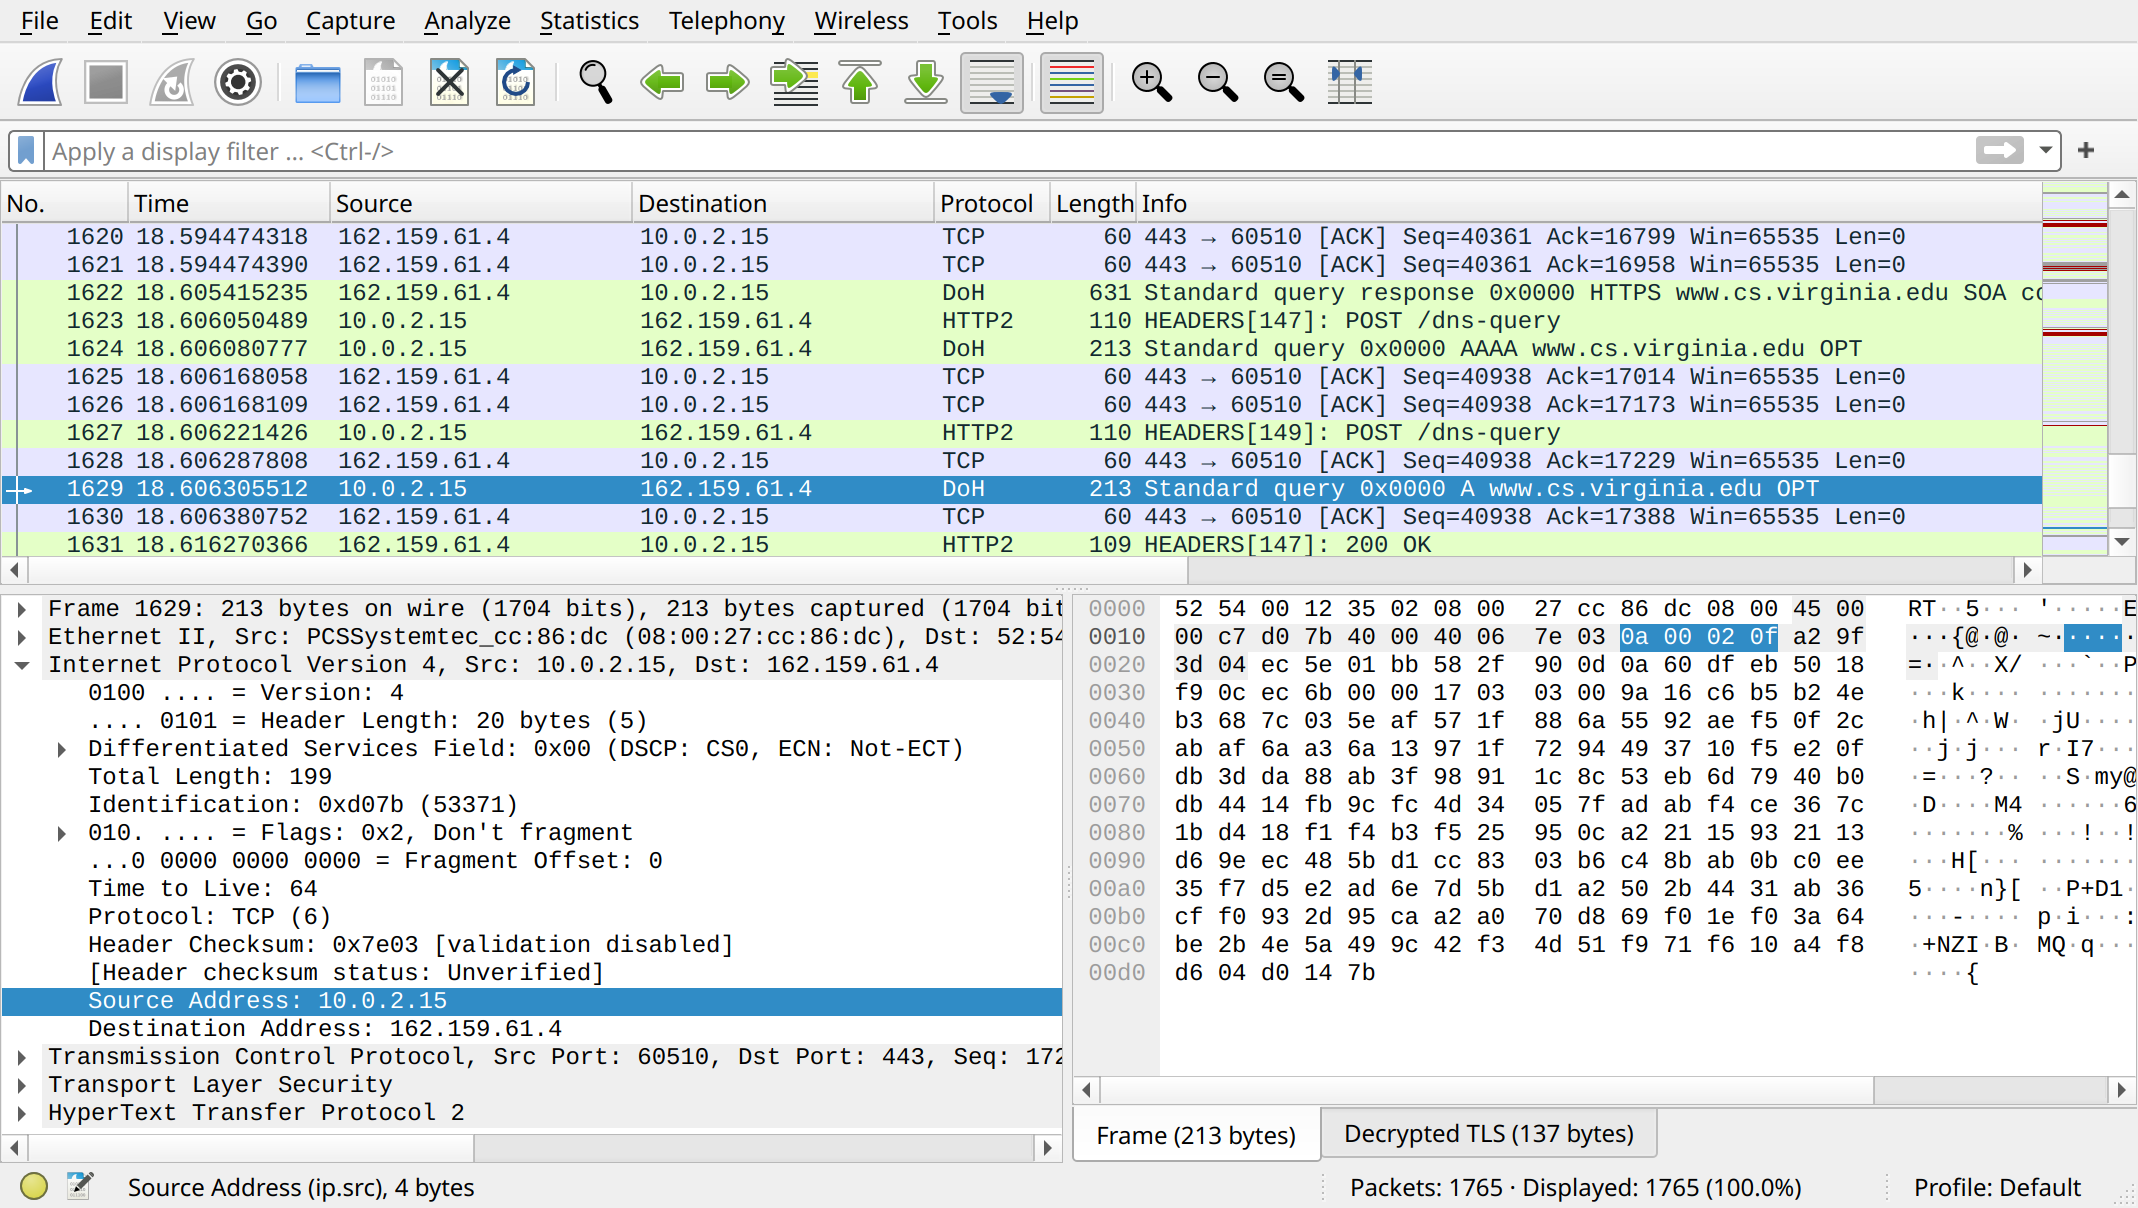
\includegraphics[width=\textwidth]{../intro/wireshark-example1.png}
};
\begin{visibleenv}<1>
    \node[text=red,overlay box] at (7.5, -2) {wireshark window};
\end{visibleenv}
\path (0, 0) rectangle (14.5, -7); % for bounding box
%\draw[overlay,help lines] (0, 0) grid (14, -8);
\begin{visibleenv}<3>
    \path[draw,red,very thick] (0, -1.2) rectangle (14.5, -4)
        node[midway,overlay box] { packet list };
    \path[draw,red,very thick] (0, -4) rectangle (7.25, -7.9)
        node[midway,overlay box] { packet details };
    \path[draw,red,very thick] (7.25, -4) rectangle (14.5, -7.9)
        node[midway,overlay box] { packet bytes };
\end{visibleenv}
\begin{visibleenv}<4>
    \path[draw,red,very thick] (0, -6.7) rectangle (7.2, -6.9);
    \path[draw,red,very thick] (10.93, -4.2) rectangle (12.1, -4.4);
    \path[draw,red,ultra thick] (7.2, -6.8) -- (10.93, -4.3)
        node[midway,above left,overlay box,align=left] {
            hilite in details \\
            shows corresponding bytes
        }
        node[midway,below right,overlay box,font=\fontsize{10}{11}\selectfont,text=black,align=left] {
            this case: \\
            \texttt{10} = \texttt{0x0a} \\
            \texttt{0} = \texttt{0x00} \\
            \texttt{2} = \texttt{0x02} \\
            \texttt{15} = \texttt{0x0f}
        };
\end{visibleenv}
\begin{visibleenv}<5>
    \path[draw,red,very thick] (6.3, -1.2) rectangle (7.15, -4);
    \node[overlay box,anchor=west] at (7.15, -3) (protocol) {`protocol'};
    \node[overlay box,font=\small,anchor=north west] at (protocol.south west) {
        the highest-layer protocol decoded
    };
\end{visibleenv}
\begin{visibleenv}<6-7>
    \begin{scope}
        \begin{pgfinterruptboundingbox}
    \tikzset{invclip/.style={clip,insert path={{[reset cm]
          (-16383.99999pt,-16383.99999pt) rectangle (16383.99999pt,16383.99999pt)
      }}}}
        \path[invclip] (6.3, -3.2) rectangle (7.15, -3.4);
        \end{pgfinterruptboundingbox}

        \fill[overlay,white,fill opacity=0.8] (0, 0) rectangle (14.5, -1.2);
        \fill[white,fill opacity=0.8] (0, -1.2) rectangle (14.5, -4);
        \fill[white,fill opacity=0.8] (7.25, -4) rectangle (14.5, -7.9);
    \end{scope}
    \path[draw,red,very thick] (0, -4) rectangle (7.25, -7.9);
    \tikzset{
        protomark/.style={Latex-,blue,thick},
        protomark brace/.style={blue,thick,decorate,decoration={brace}},
        protomark label/.style={blue,fill=white,fill opacity=0.9},
    }
    \draw[protomark] (7.25, -4.3) -- ++(1, 0) node[right,protomark label] {ethernet};
    \draw[protomark brace] (7.3, -4.5) -- (7.3, -7.1);
        \draw[protomark] (7.4, -5.8) -- ++ (0.75, .6) node[right, protomark label] {
                IPv4 (internet protocol version 4)
        };
    \draw[protomark] (7.25, -7.2) -- ++(1, 1) node[right,protomark label] {
        TCP ({\fontsize{10}{11}\selectfont transmission control protocol})
    };
    \draw[protomark] (7.25, -7.325) -- ++(1, .5) node[right,protomark label] {
        TLS ({\fontsize{10}{11}\selectfont transport layer security})
    };
    \draw[protomark] (7.25, -7.45) -- ++(1, -.2) node[right,protomark label] {
        HTTP/2 ({\fontsize{10}{11}\selectfont hypertext transfer protocol 2})
    };
\end{visibleenv}
\begin{visibleenv}<7>
    \draw[red, very thick] (6.3, -3.2) rectangle (7.15, -3.4);
    \draw[red,Latex-,very thick] (7.15, -3.3) -- ++(1, 0) node[right,align=left,overlay box] {
        DoH is not \\one of these!
    };
\end{visibleenv}
\end{tikzpicture}
\end{frame}

\begin{frame}{}
\begin{tikzpicture}
\tikzset{
    overlay box/.style={fill=white,fill opacity=0.9}
}
\node[overlay,anchor=north west,inner sep=0mm] (base) at (0, 0) {
    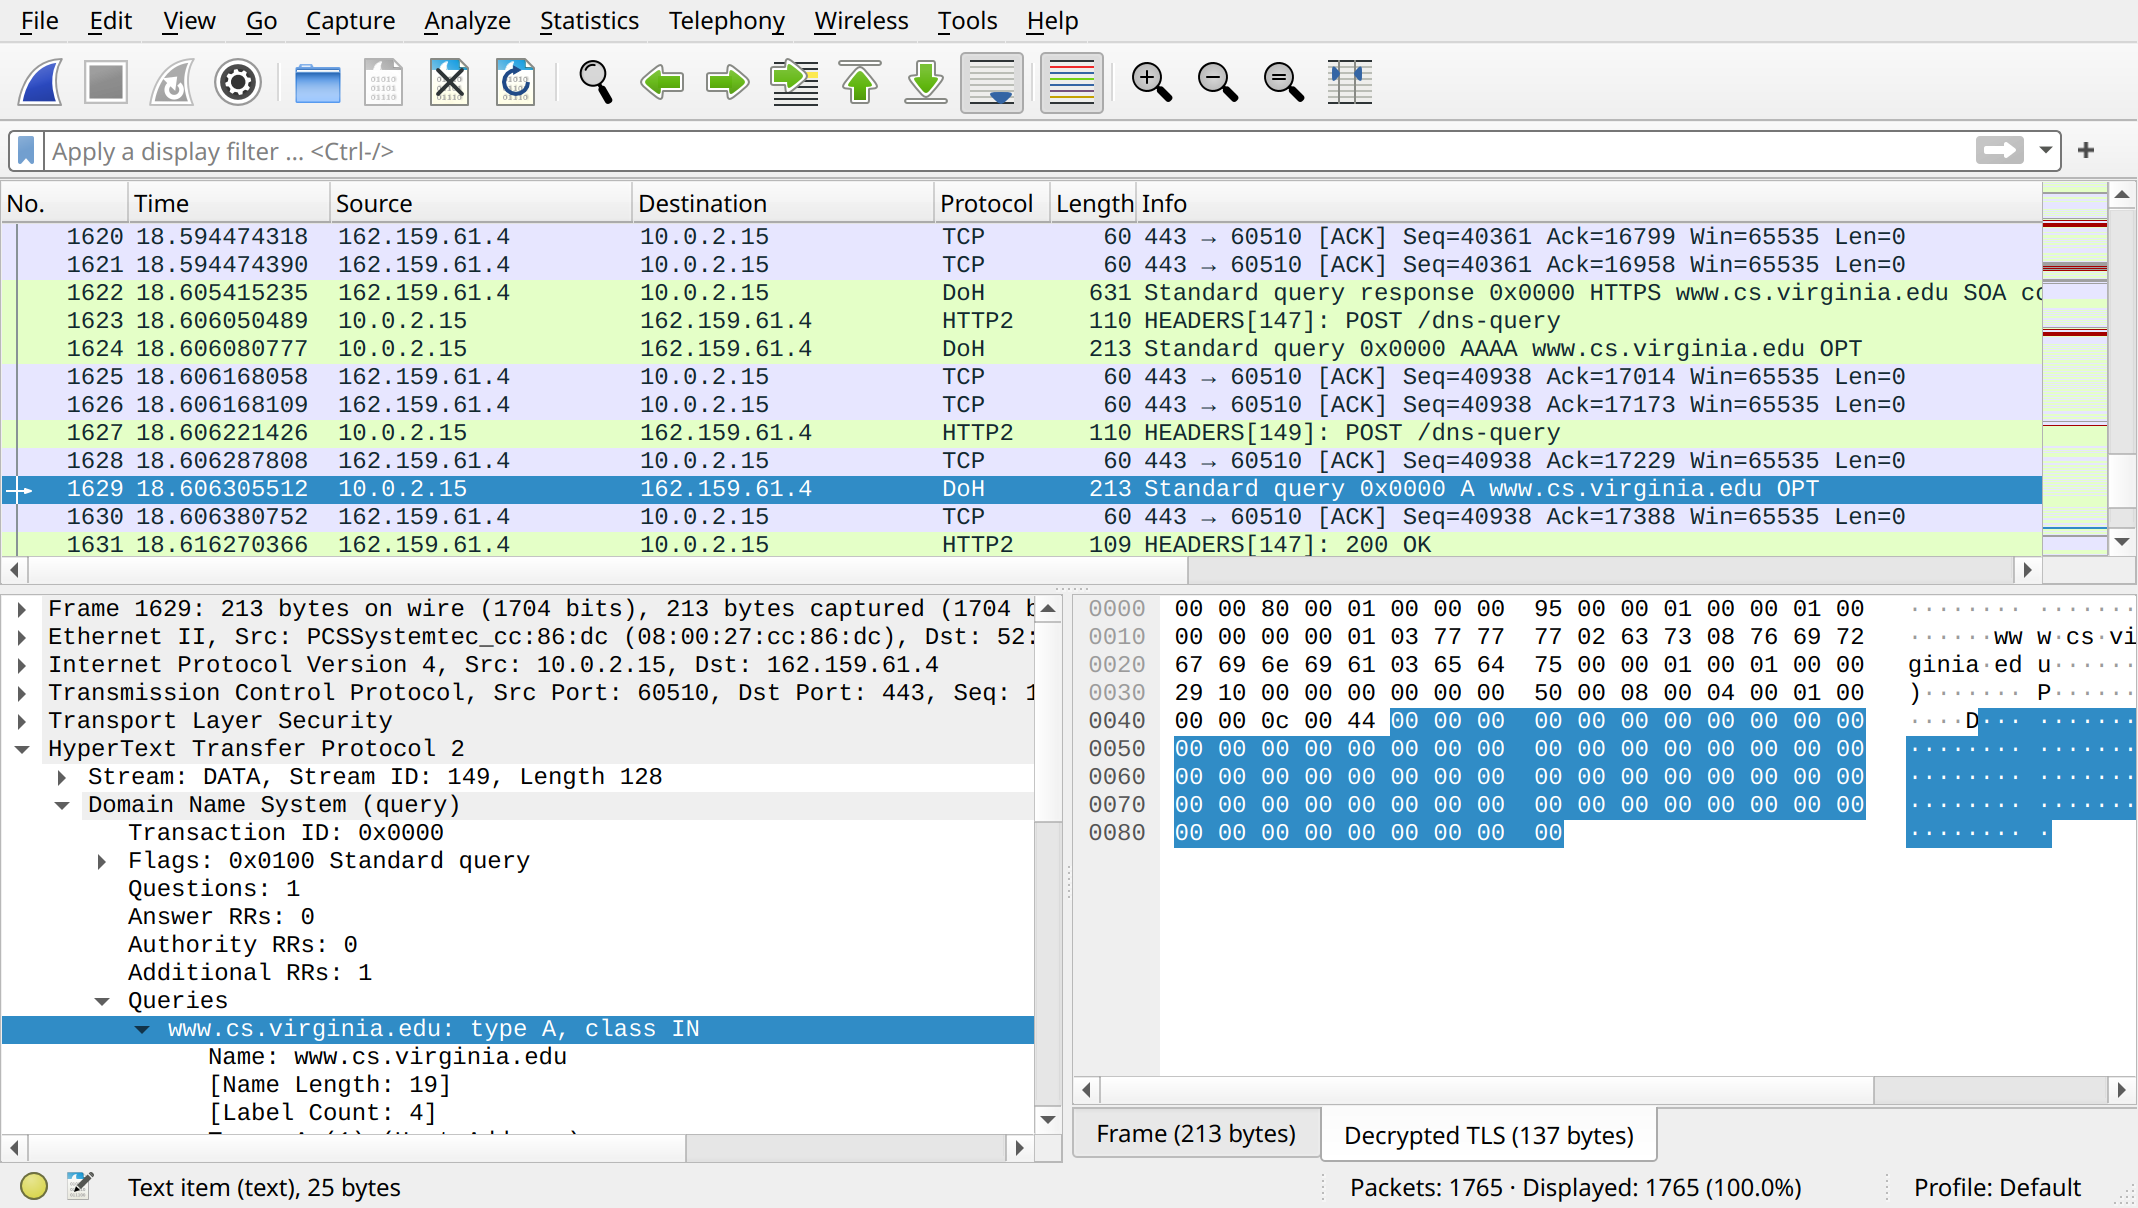
\includegraphics[width=\textwidth]{../intro/wireshark-doh-zoom.png}
};
\path (0, 0) rectangle (14.5, -7); % for bounding box
%\draw[overlay,help lines] (0, 0) grid (14, -8);
    \begin{scope}
        \begin{pgfinterruptboundingbox}
    \tikzset{invclip/.style={clip,insert path={{[reset cm]
          (-16383.99999pt,-16383.99999pt) rectangle (16383.99999pt,16383.99999pt)
      }}}}
        \path[invclip] (6.3, -3.2) rectangle (7.15, -3.4);
        \end{pgfinterruptboundingbox}

        \fill[overlay,white,fill opacity=0.8] (0, 0) rectangle (14.5, -1.2);
        \fill[white,fill opacity=0.8] (0, -1.2) rectangle (14.5, -4);
        \fill[white,fill opacity=0.8] (7.25, -4) rectangle (14.5, -7.9);
    \end{scope}
    \path[draw,red,very thick] (0, -4) rectangle (7.25, -7.9);
    \tikzset{
        protomark/.style={Latex-,blue,thick},
        protomark alt/.style={Latex-,violet,thick,dotted},
        protomark brace/.style={blue,thick,decorate,decoration={brace}},
        protomark brace alt/.style={violet,thick,decorate,decoration={brace}},
        protomark label/.style={blue,fill=white,fill opacity=0.9},
    }
    \draw[protomark] (7.25, -4.3) -- ++(1, .2) node[right,protomark label] {ethernet};
    \draw[protomark] (7.25, -4.5) -- ++ (1, -.2) node[right, protomark label] {
                IPv4 (internet protocol version 4)
        };
    \draw[protomark] (7.25, -4.6) -- ++(1, -.6) node[right,protomark label] {
        TCP ({\fontsize{10}{11}\selectfont transmission control protocol})
    };
    \draw[protomark] (7.25, -4.8) -- ++(1, -1) node[right,protomark label] {
        TLS ({\fontsize{10}{11}\selectfont transport layer security})
    };
    \draw[protomark brace] (7.3, -5) -- (7.3, -7.9);
        \draw[protomark] (7.4, -6.5) -- ++ (0.75, 0) node[right, protomark label] {
            HTTP/2 ({\fontsize{10}{11}\selectfont hypertext transfer protocol 2})
        };
    \draw[protomark brace alt] (7.5, -5.5) -- (7.5, -7.9);
        \draw[protomark alt] (7.6, -6.85) -- ++ (0.75, -.5) node[right, protomark label] {
            DNS (domain name system)
        };
    \draw[red, very thick] (6.3, -3.2) rectangle (7.15, -3.4);
    \draw[red,Latex-,very thick] (7.15, -3.3) -- ++(1, 0) node[right,align=left,overlay box] {
        DoH = DNS over HTTPS
    };
\end{tikzpicture}
\end{frame}

\begin{frame}[fragile]{}
\providecommand{\doHilite}[6]{
    %\doHilite{Y offset start protocol list}{Y offset end protocol list}
    %         {X offset corner data}{Y offset corner data}
    %         {X offset other corner data}{Y offset other corner data}
    \path[draw,red,very thick] (0, -3.95 - #1 * 0.206) rectangle (7.25, -3.95 - #2 * 0.206);
    \path[draw,red,very thick] (7.95 + #3, -4.2059 - #4 * 0.2059) -- (7.95 + #3, -3.95 - #4 * 0.2059)
            -- (12.8, -3.95 - #4 * 0.2059)
            |- (7.95 + #5, -4 - #6 * 0.2059) 
            |- (7.95, -4 - #6 * 0.2059 - .2059) |- cycle;
}
\providecommand{\doHiliteOneDataLine}[6]{
    %\doHilite{Y offset start protocol list}{Y offset end protocol list}
    %         {X offset corner data}{Y offset corner data}
    %         {X offset other corner data}{Y offset other corner data}

    \path[draw,red,very thick] (0, -3.95 - #1 * 0.207) rectangle (7.25, -4 - #2 * 0.207);
    \path[draw,red,very thick] (7.95 + #3, -4.207 - #4 * 0.207) -- (7.95 + #3, -4 - #4 * 0.207)
            %-- (12.8, -4 - #4 * 0.207)
            |- (7.95 + #5, -4 - #6 * 0.207) 
            |- (7.95, -4 - #6 * 0.207 - .207) |- cycle;
}
\begin{tikzpicture}
\tikzset{
    overlay box/.style={fill=white,fill opacity=0.9},
}
\node[overlay,anchor=north west,inner sep=0mm] (base) at (0, 0) {%
\only<1-2>{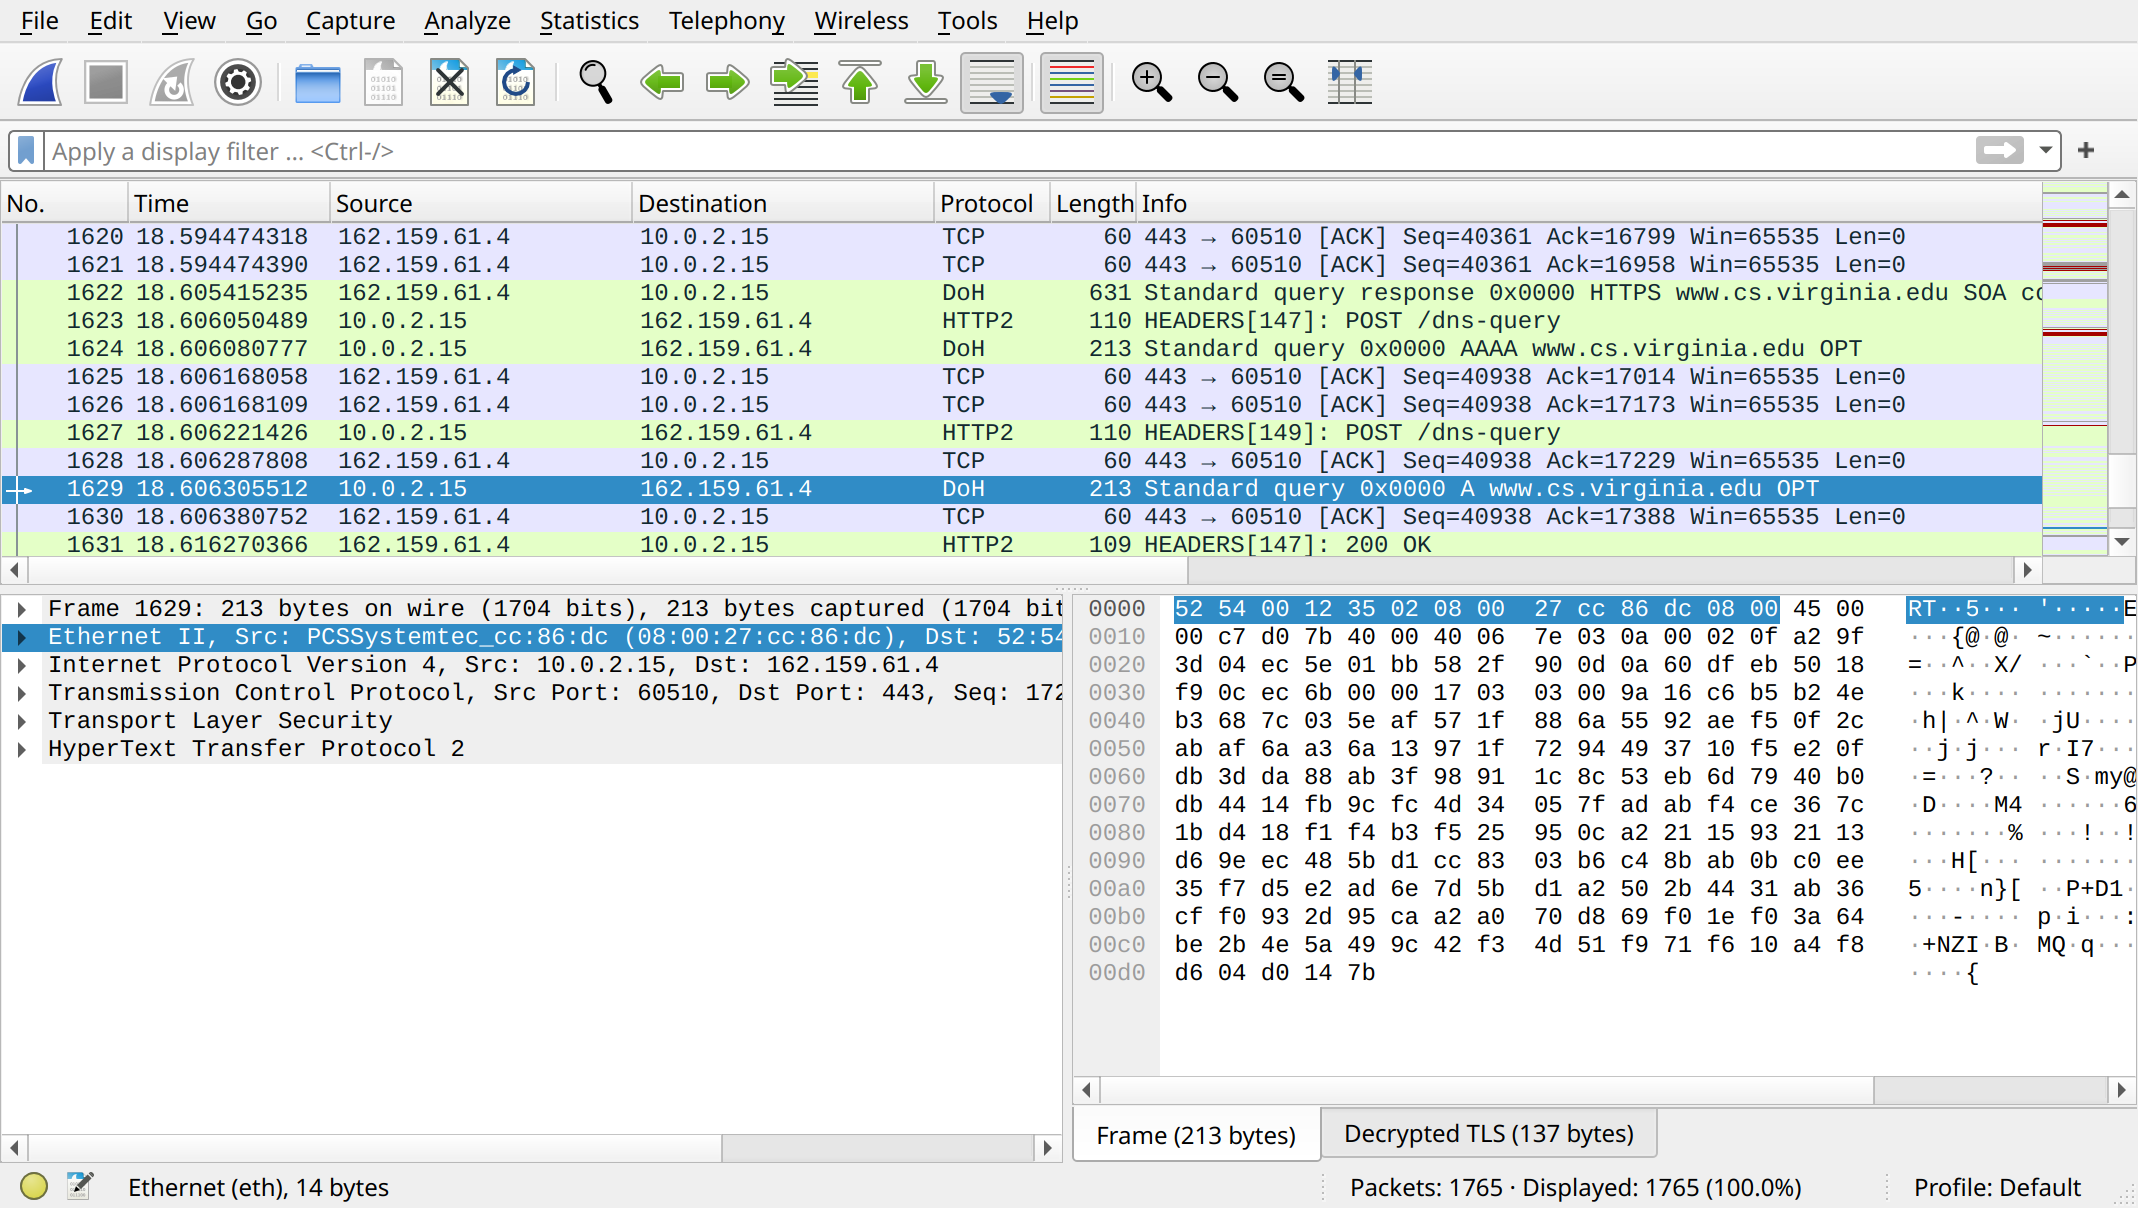
\includegraphics[width=\textwidth]{../intro/wireshark-hi-ethernet.png}}%
\only<3-4>{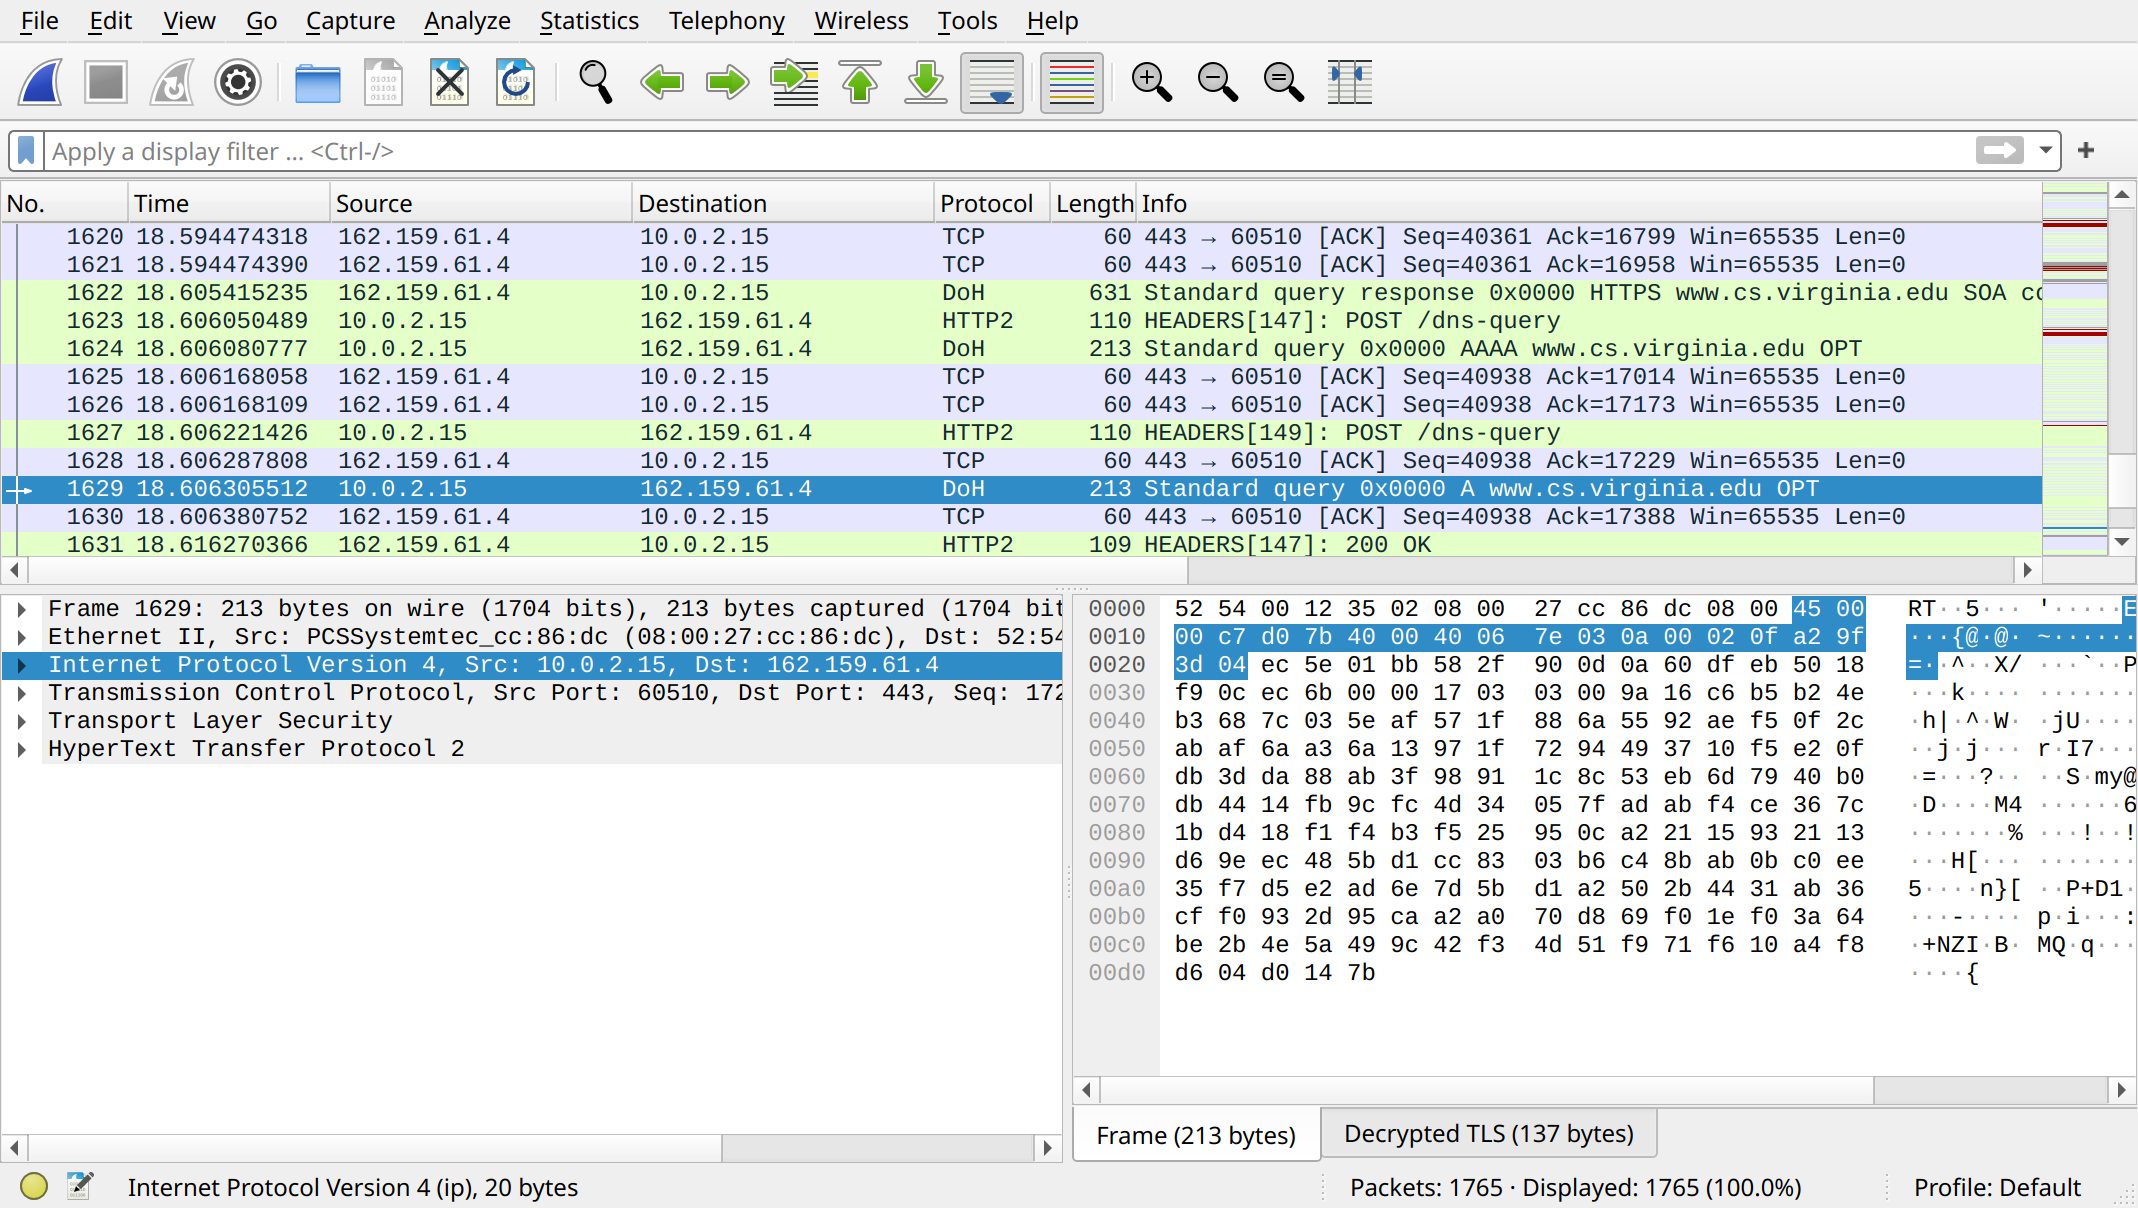
\includegraphics[width=\textwidth]{../intro/wireshark-hi-ipv4.png}}%
\only<5-6>{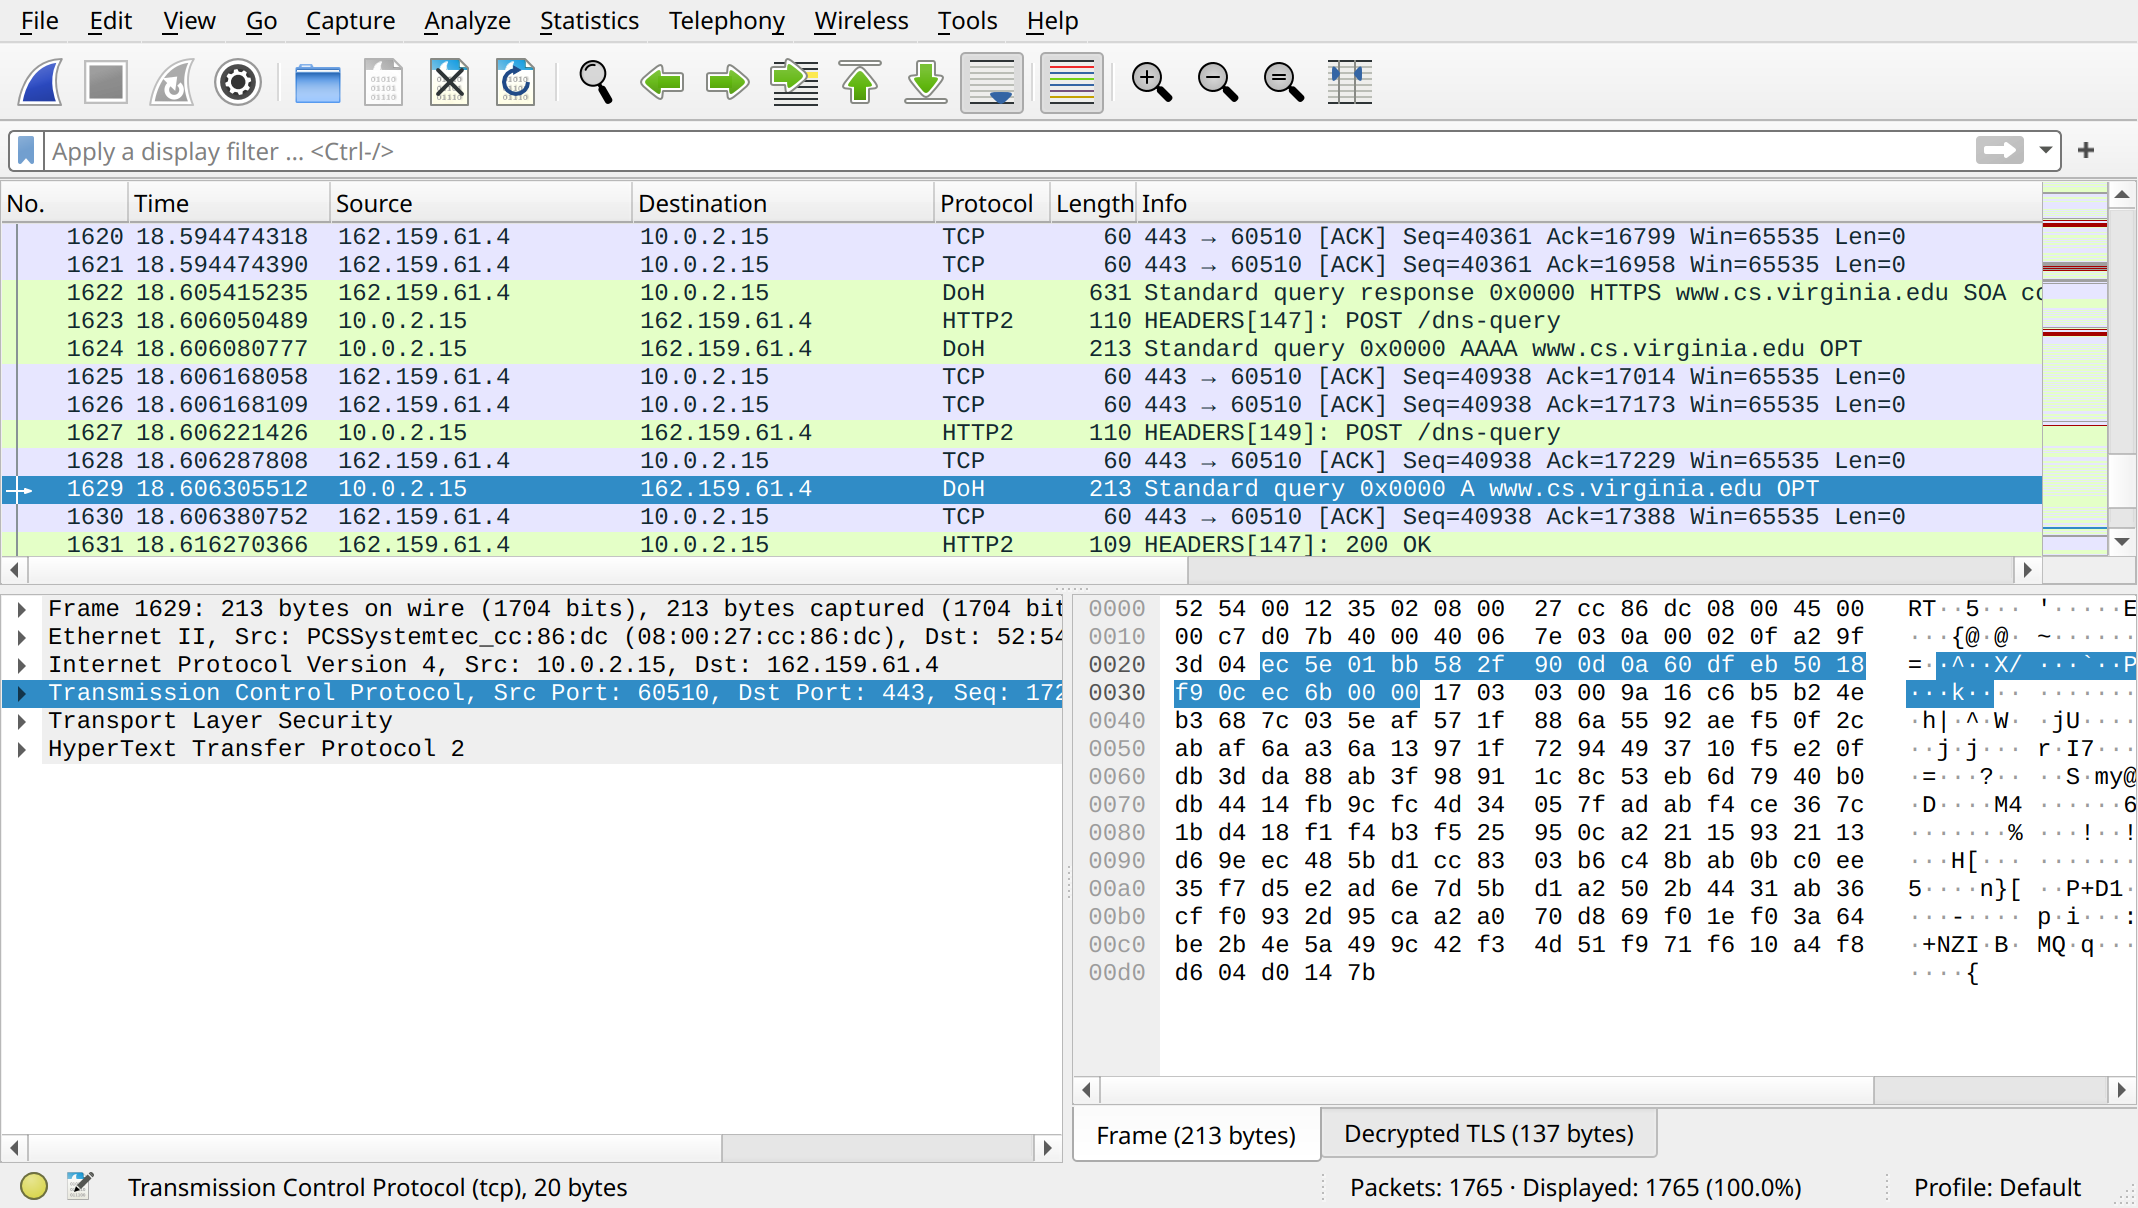
\includegraphics[width=\textwidth]{../intro/wireshark-hi-tcp.png}}%
\only<7-8>{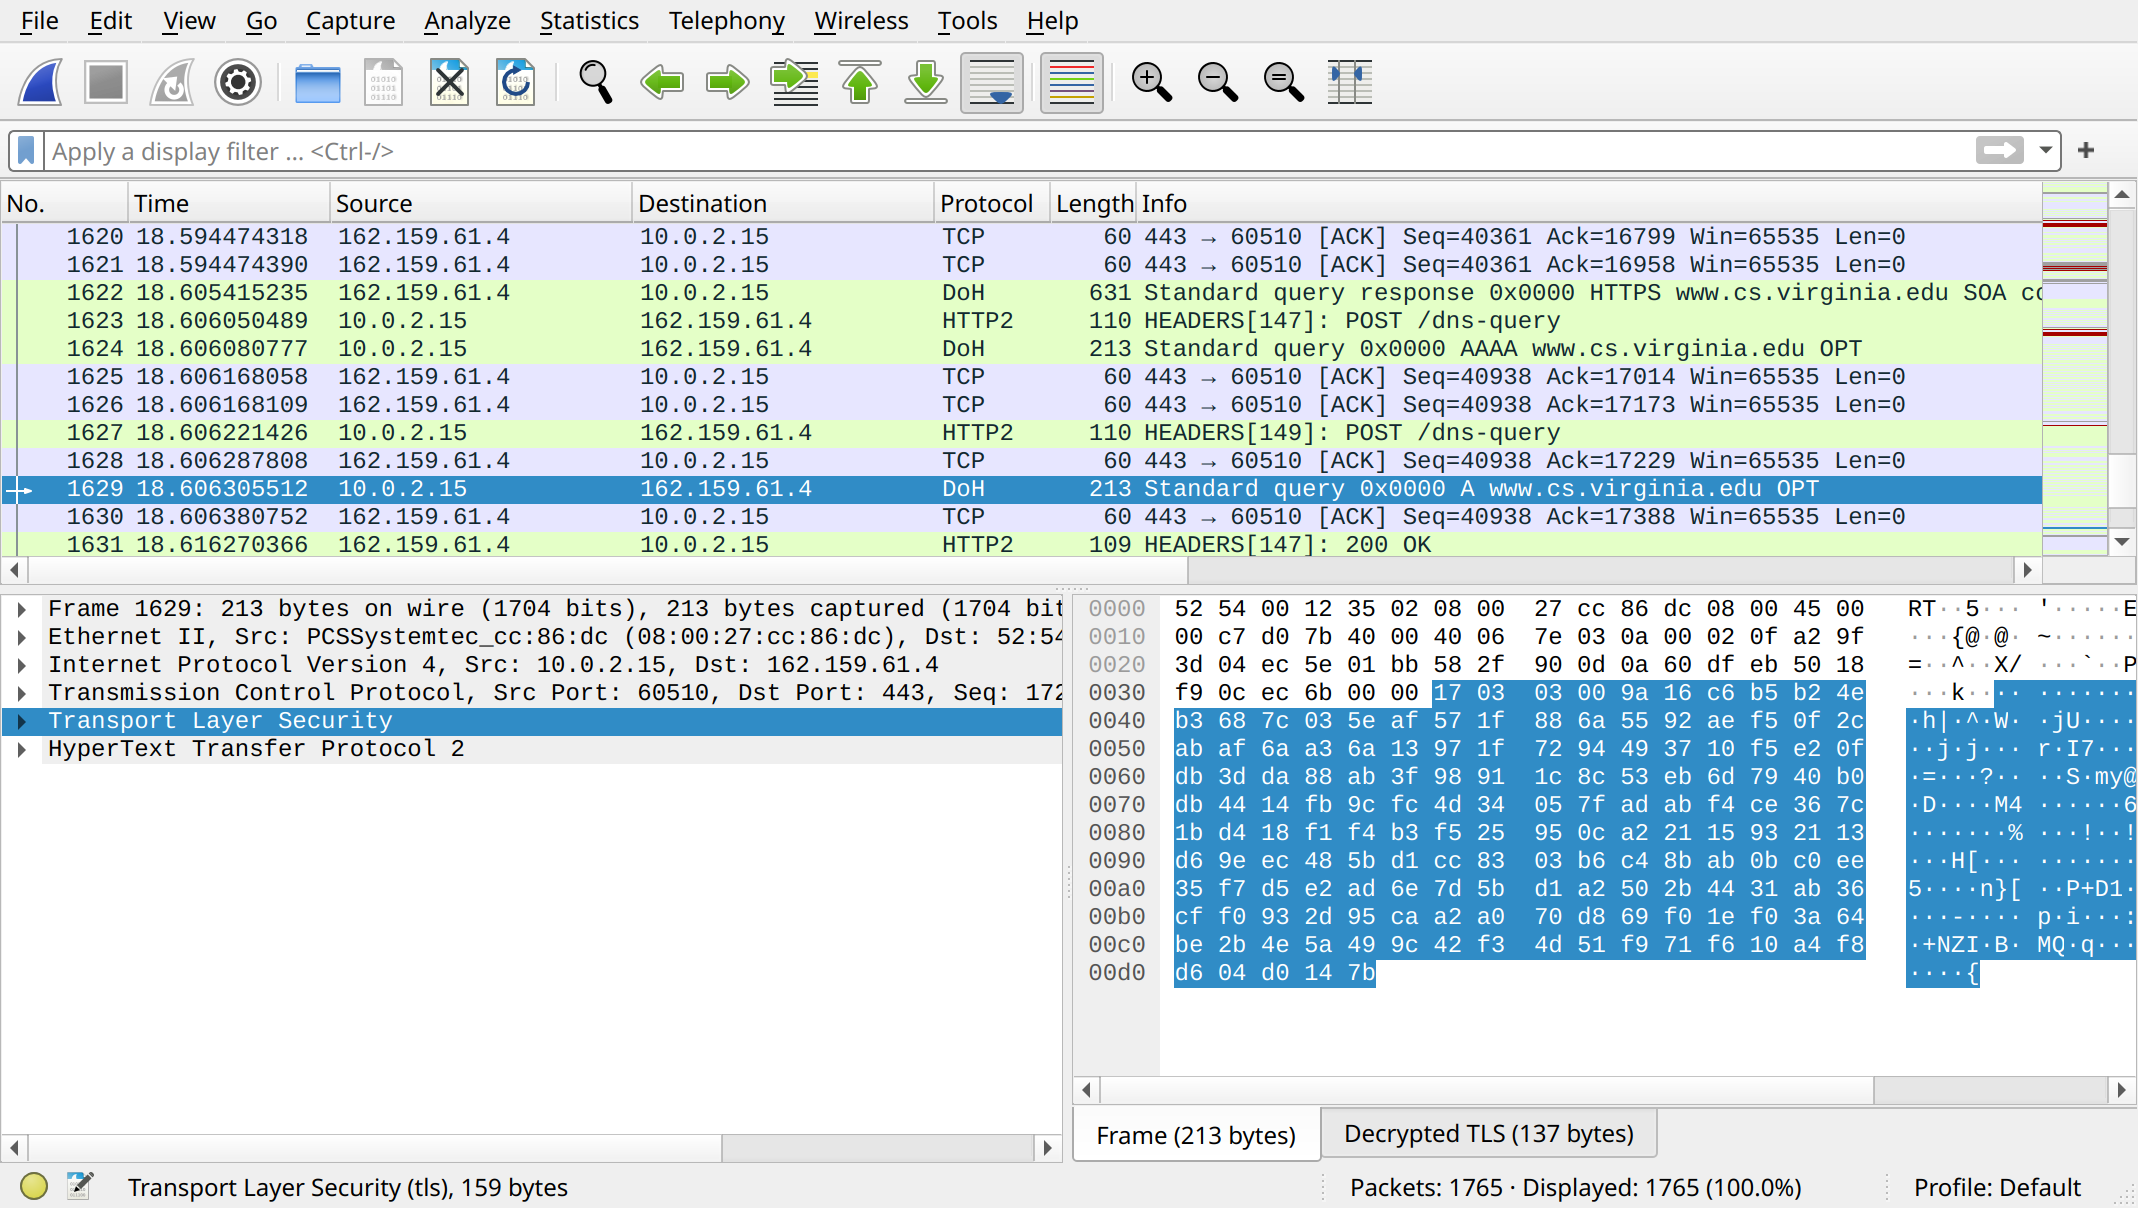
\includegraphics[width=\textwidth]{../intro/wireshark-hi-tls.png}}%
\only<9-11>{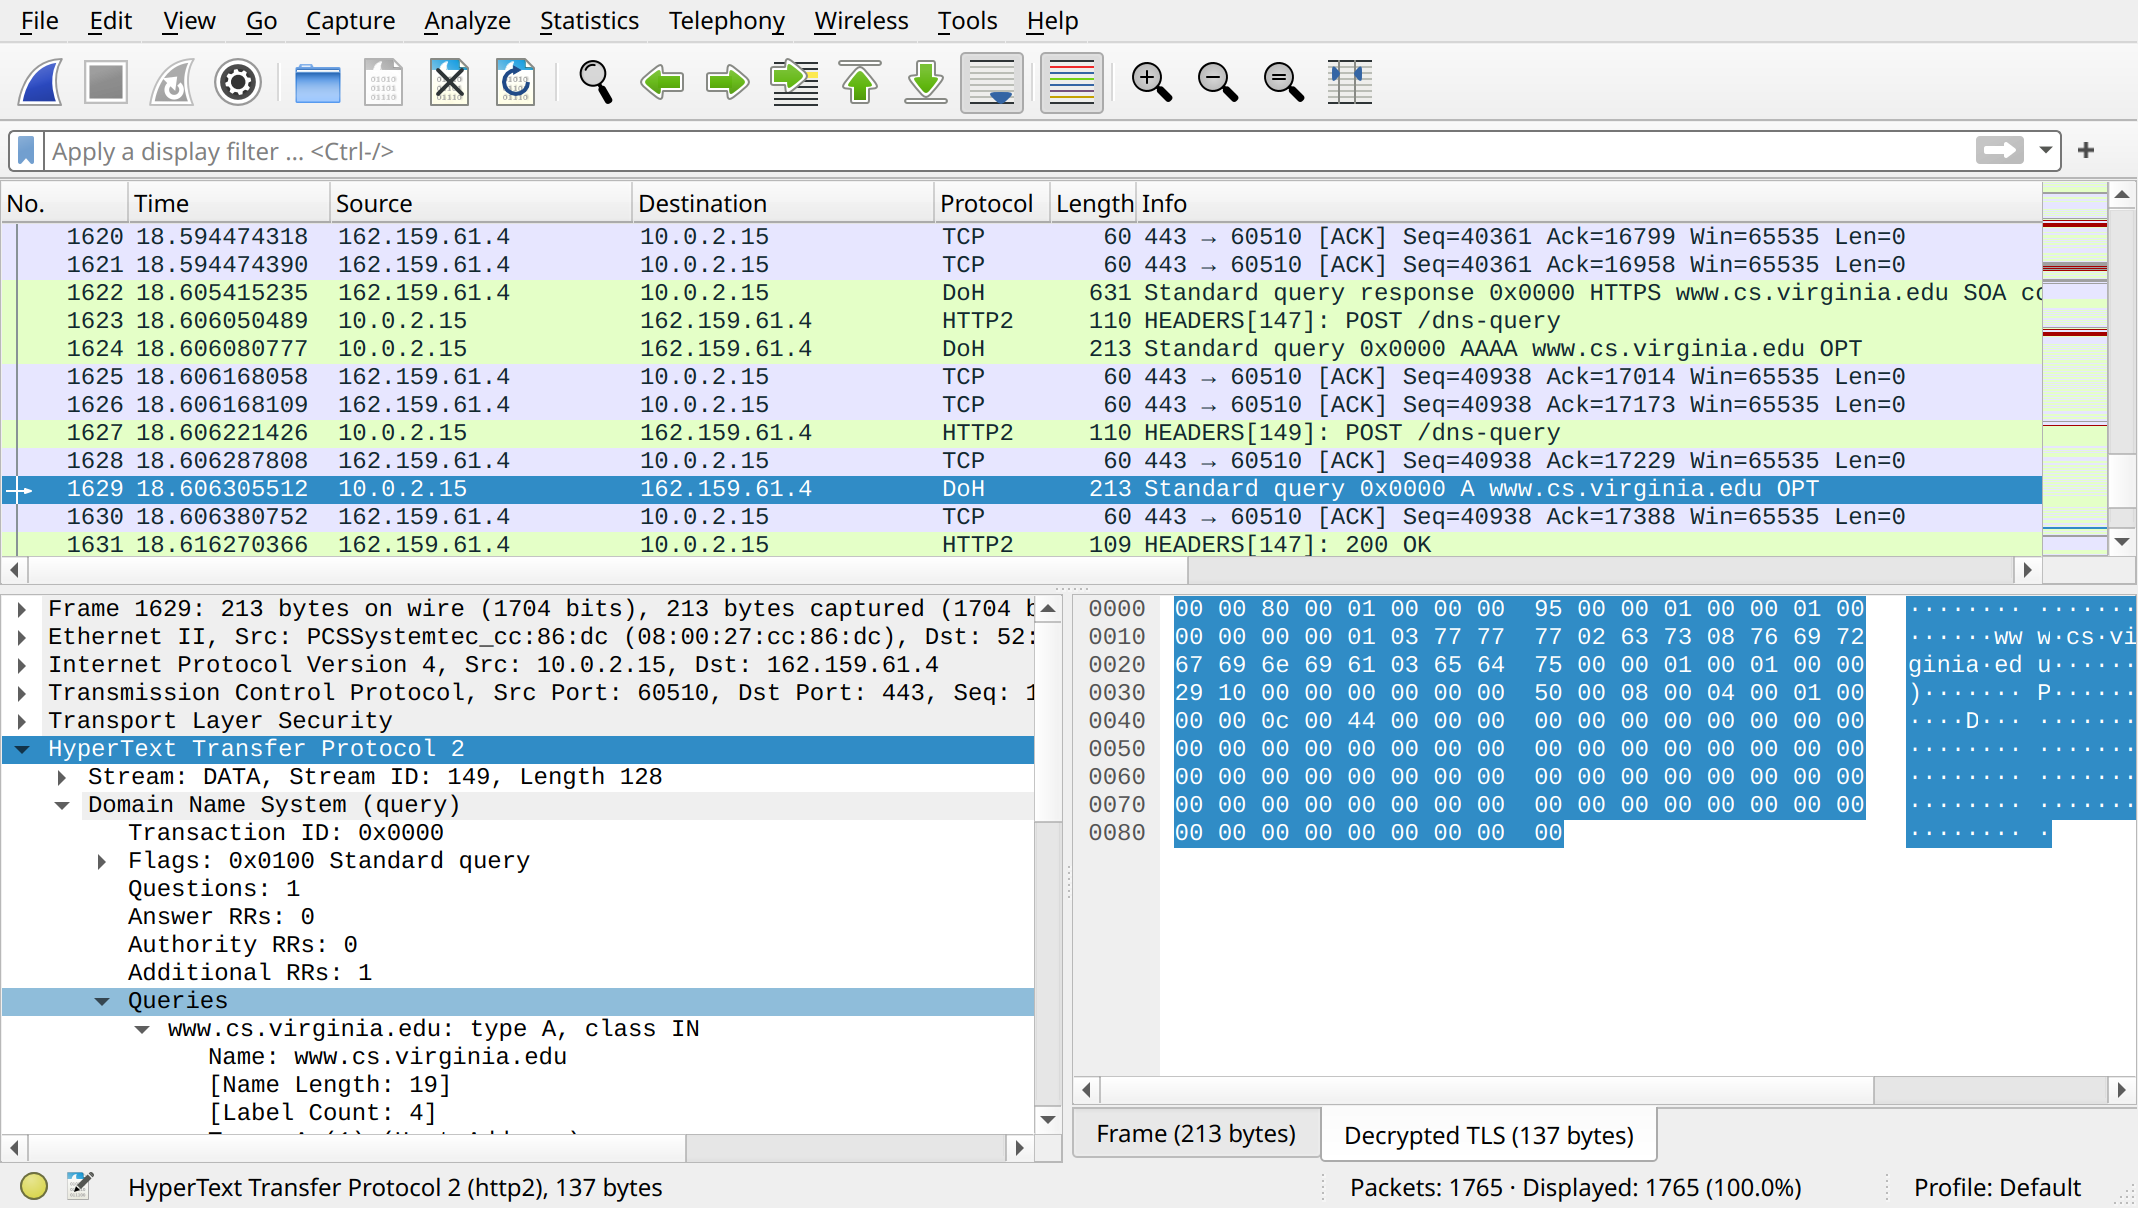
\includegraphics[width=\textwidth]{../intro/wireshark-hi-http.png}}%
\only<12-13>{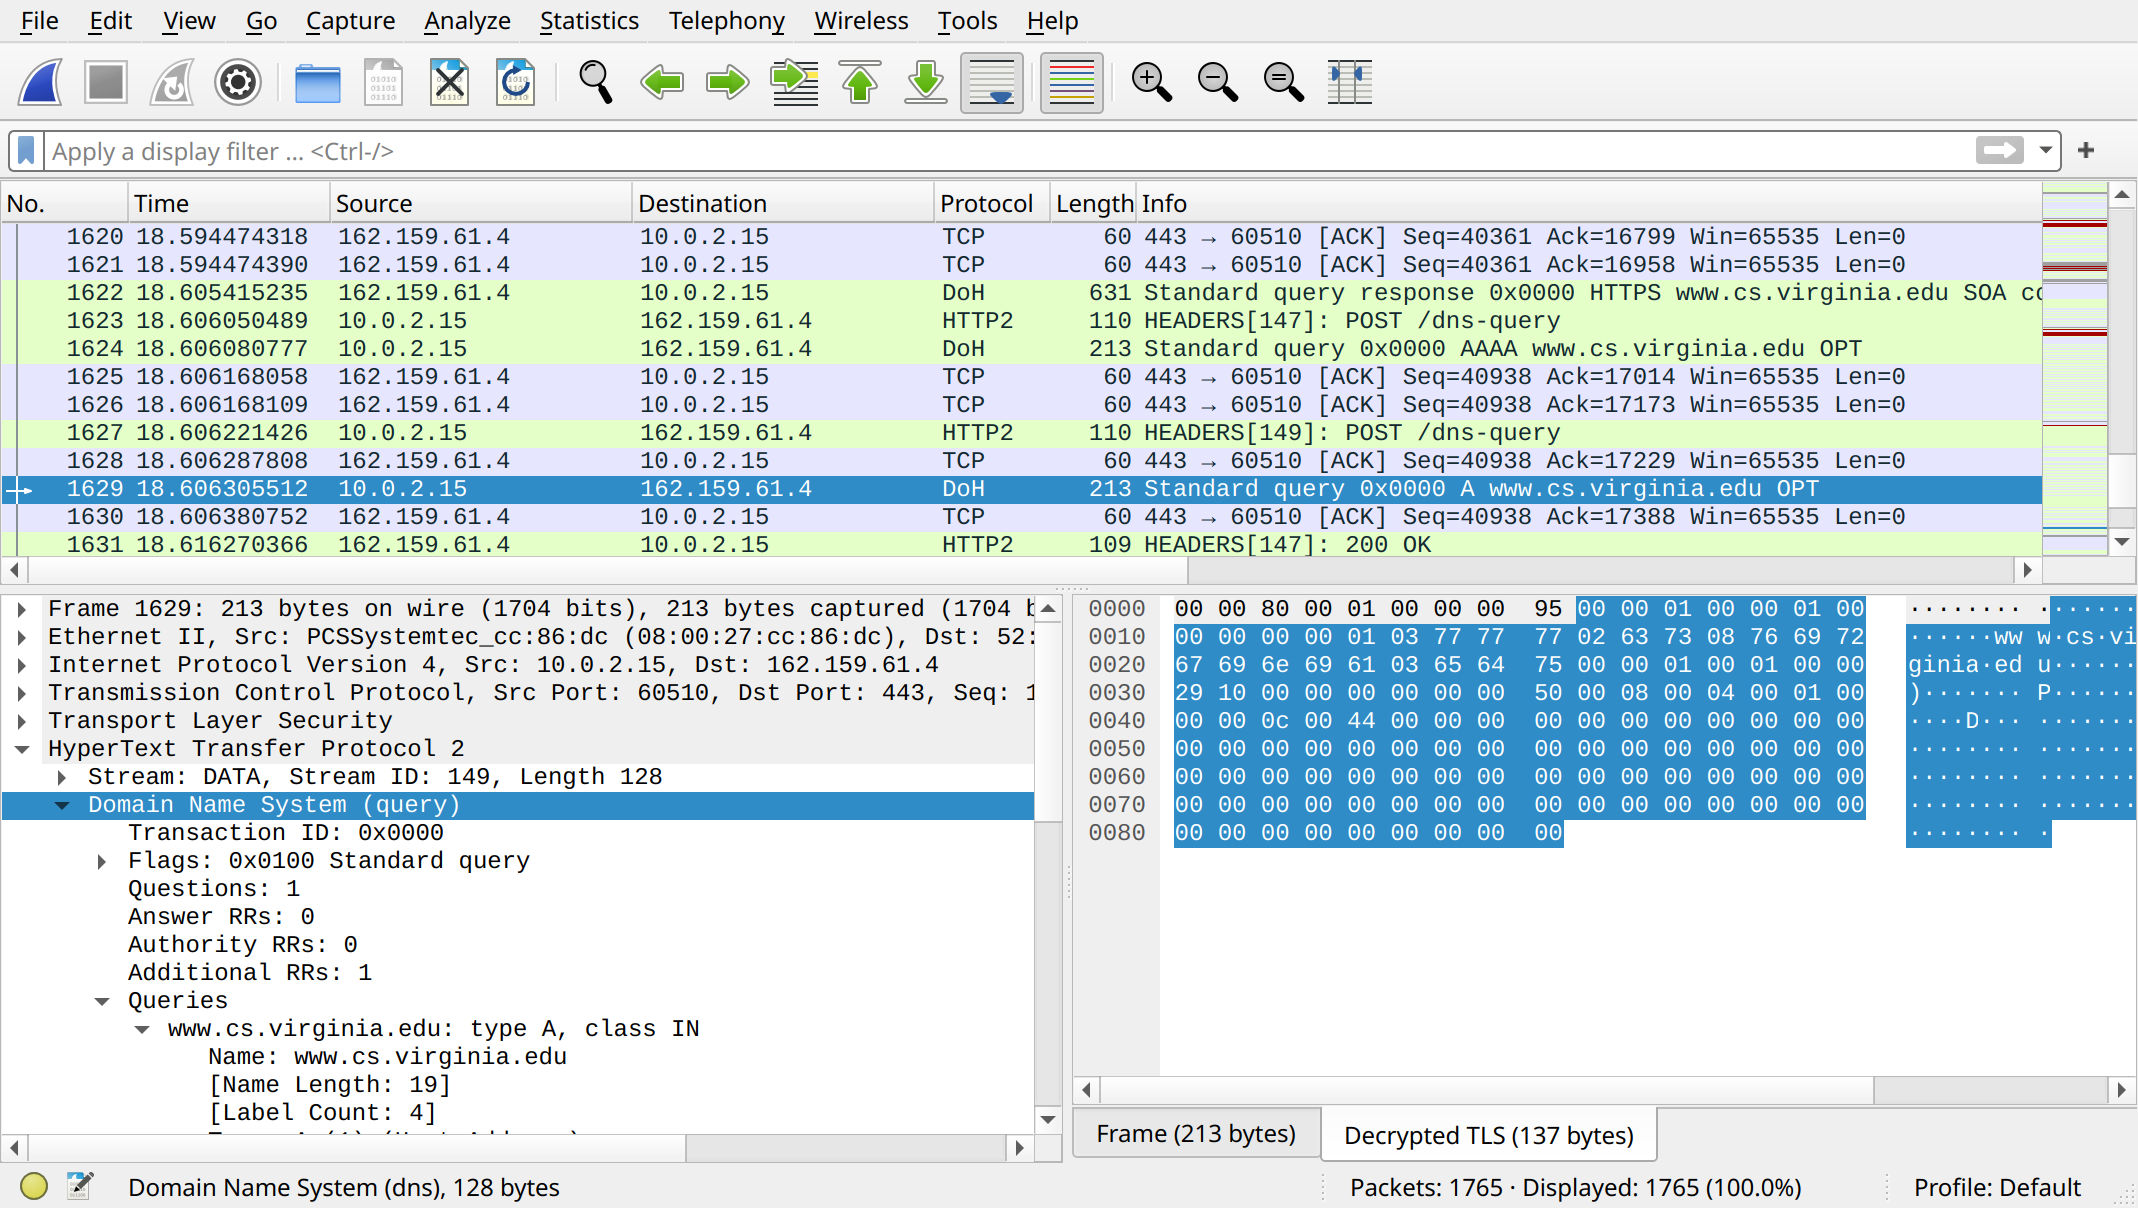
\includegraphics[width=\textwidth]{../intro/wireshark-hi-dns-in-tls.png}}%
};
%\draw[overlay,help lines] (0, 0) grid (14, -8);
\path (0, 0) rectangle (14.5, -7); % for bounding box

\begin{visibleenv}<1> % ethernet
    \doHiliteOneDataLine{1}{2}{0}{0}{4.2}{0}
\end{visibleenv}
\begin{visibleenv}<3> % IP
    \doHilite{2}{3}{4.2}{0}{0.5}{2}
\end{visibleenv}
\begin{visibleenv}<5> % TCP
    \doHilite{3}{4}{0.5}{2}{1.7}{3}
\end{visibleenv}
\begin{visibleenv}<7> % TLS
    \doHilite{4}{5}{1.7}{3}{1.4}{12}
\end{visibleenv}
\begin{visibleenv}<9> % HTTP, decrypted TLS
    \path[draw,red,very thick] (8.9, -7.5) rectangle (11.3, -7.9);
    \node[align=left,overlay box,anchor=south] at (10.4, -7.5) {
        setup step: got Firefox to output \\
        cryptographic keys ({\fontsize{10}{11}\selectfont using \tt SSLKEYLOGFILE})
    };
\end{visibleenv}
\begin{visibleenv}<10> % HTTP
    \doHilite{5}{6}{0}{0}{2.69}{8}
\end{visibleenv}
\begin{visibleenv}<12> % DNS
    \doHilite{7}{8}{2.7}{0}{2.69}{8}
\end{visibleenv}
\end{tikzpicture}
\end{frame}

% FIXME: show multiple related packets --- emphasize filter window
\begin{frame}{}
\begin{tikzpicture}
\tikzset{
    overlay box/.style={fill=white,fill opacity=0.9}
}
\node[overlay,anchor=north west,inner sep=0mm] (base) at (0, 0) {
    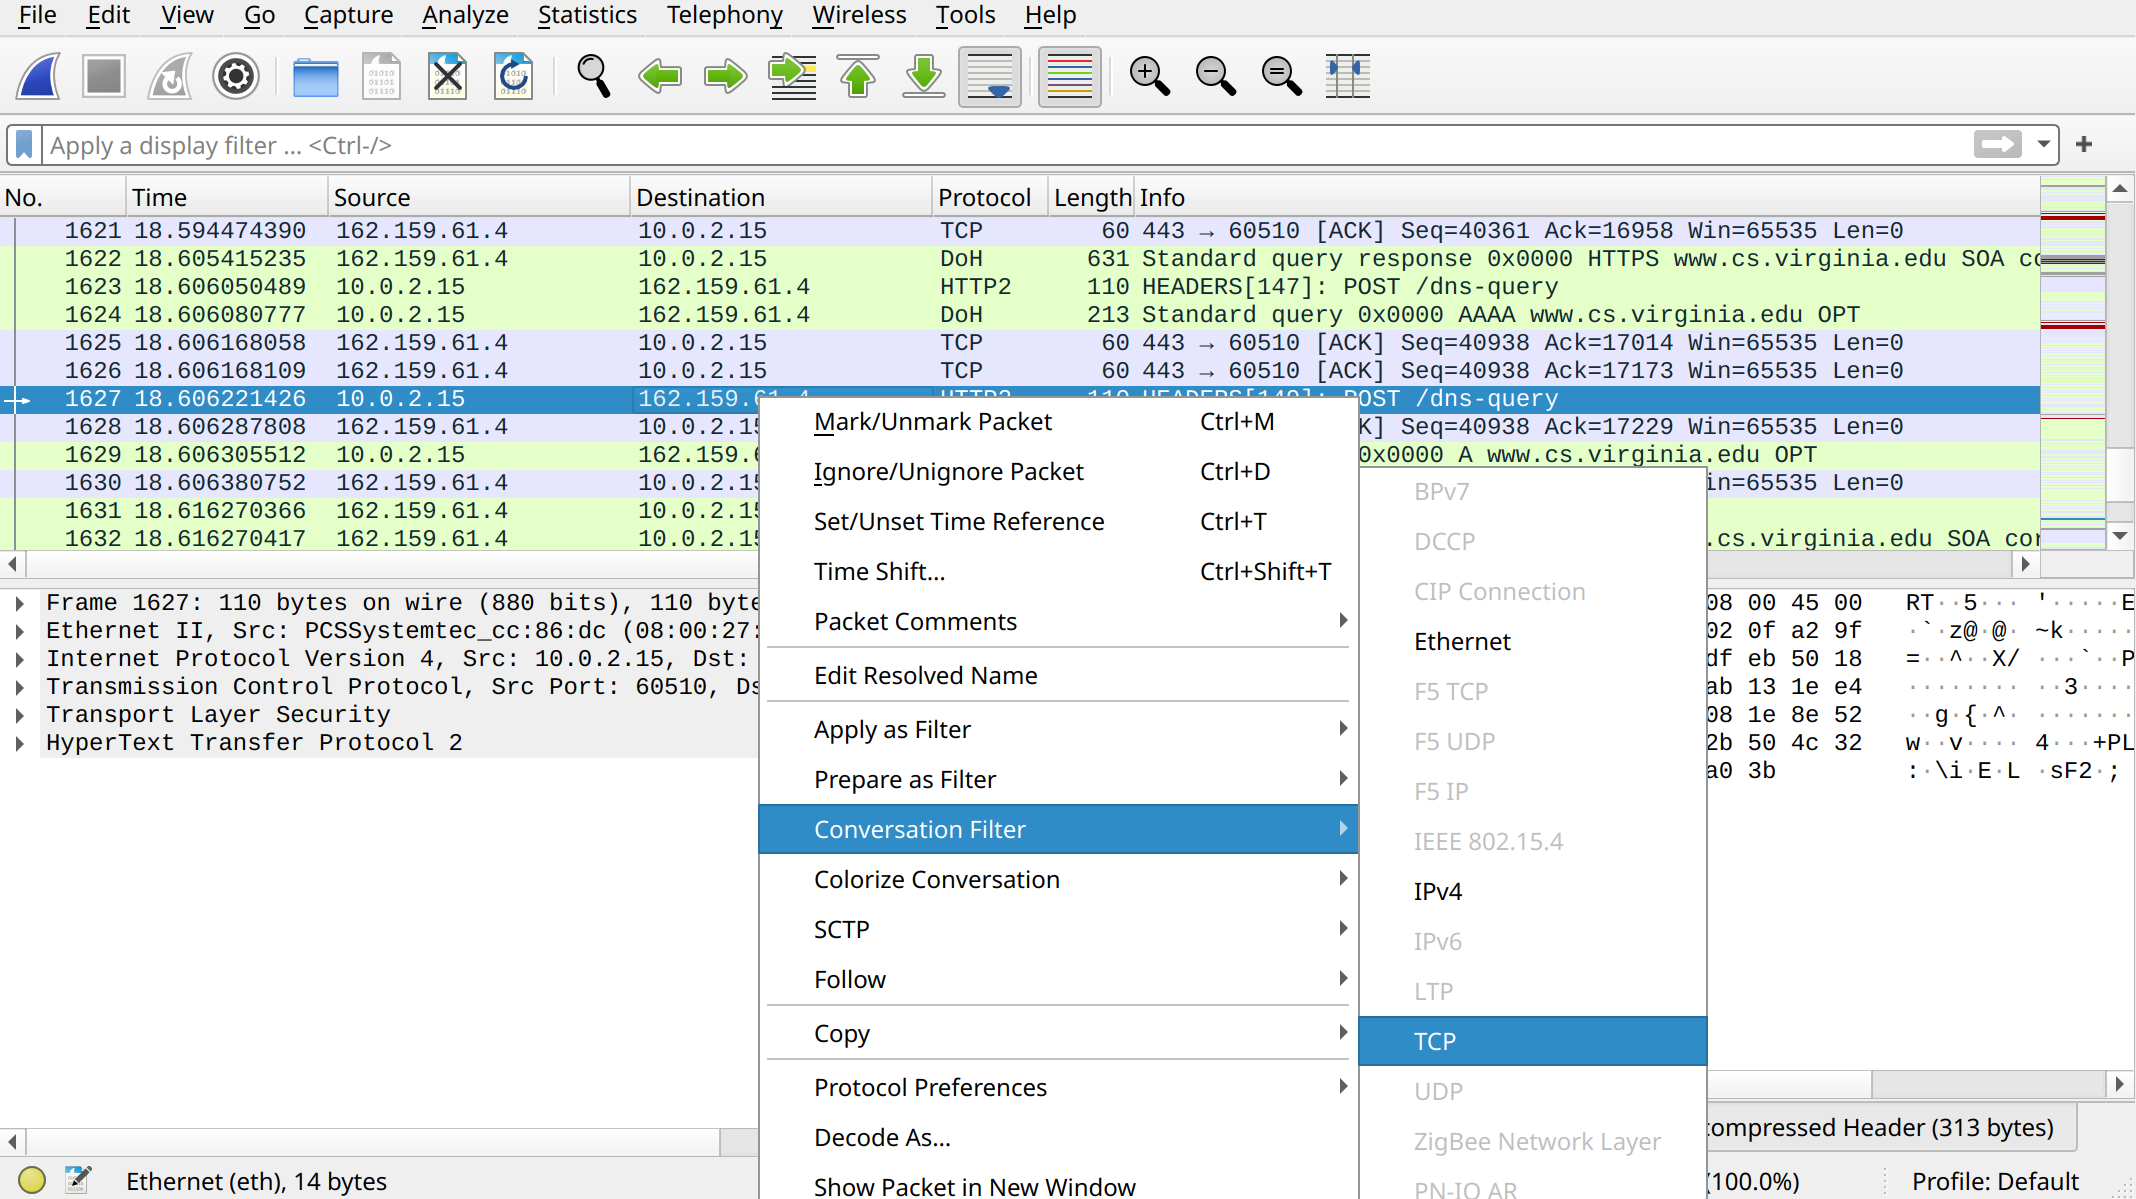
\includegraphics[width=\textwidth]{../intro/wireshark-menu-tcp-filter.png}
};
\path (0, 0) rectangle (14.5, -7); % for bounding box
\end{tikzpicture}
\end{frame}

\begin{frame}{}
\begin{tikzpicture}
\tikzset{
    overlay box/.style={fill=white,fill opacity=0.9}
}
\node[overlay,anchor=north west,inner sep=0mm] (base) at (0, 0) {
    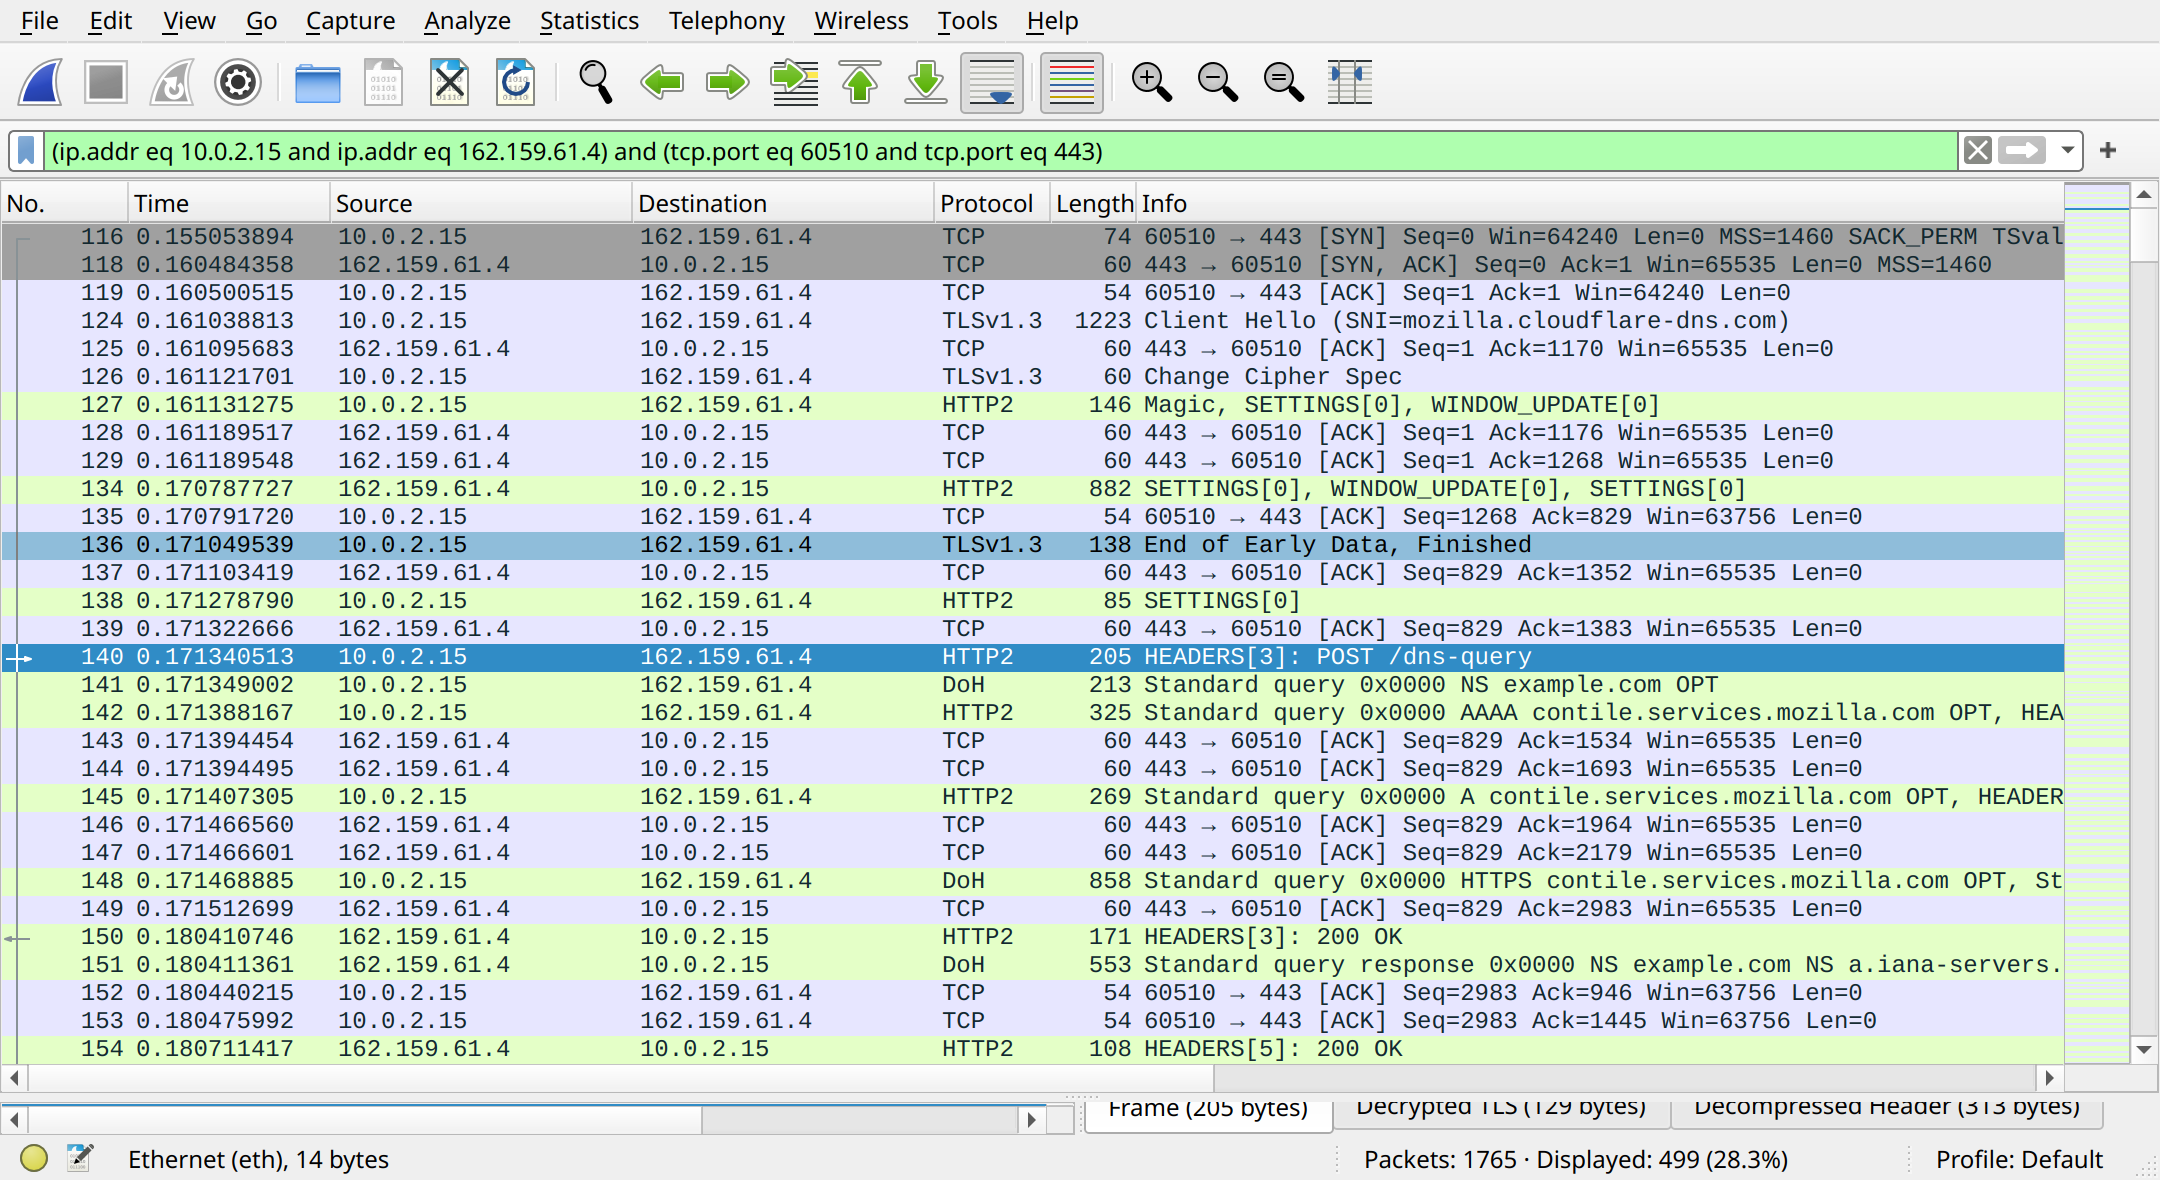
\includegraphics[width=\textwidth]{../intro/wireshark-filtered.png}
};
\path (0, 0) rectangle (14.5, -7); % for bounding box
%\draw[overlay,help lines] (0, 0) grid (14, -8);
%\draw[overlay,help lines,dotted] (0, 0) grid[step=0.2] (14, -8);
\begin{visibleenv}<1>
    \path[draw, red, very thick] (0.3, -0.9) rectangle (13.15, -1.15);
    \node[anchor=north,overlay box,text=red] (filter expr label) at (6.5, -1.15) {
        filter expression 
    };
    \node[anchor=north,overlay box,font=\fontsize{10}{11}\selectfont,align=left] at (filter expr label.south) {
        based on address ($\sim$ machine) and port number ($\sim$ program/socket) fields  \\
        usually means all part of one socket connection
    };
    \path[draw, red, very thick] (10.3, -7.6) rectangle (12.1, -7.9);
    \node[anchor=south,overlay box,text=red] at (11.4, -7.6) {
        499 packets in ``conversation''
    };
\end{visibleenv}
\begin{visibleenv}<2>
    \path[draw,red, very thick] (0, -1.9) rectangle (.85, -2.24);
    \path[draw,red, very thick] (0, -3) rectangle (.85, -3.37);
    \node[overlay box,anchor=west,text=red] at (.85, -2.5) {
        some packets not shown from filter
    };
\end{visibleenv}
\begin{visibleenv}<3>
    \path[draw,red,very thick] (6.25, -1.47) rectangle (7.1, -7.2);
    \node[align=left,overlay box,anchor=south east,text=red] at (6.25, -3) {
        highest layer used \\
        in each packet
    };
    \node[align=left,overlay box,anchor=north east,text=black,font=\fontsize{10}{11}] at (6.25, -3) {
        connection only `for' \\
        DNS over HTTPS (DoH) \\
        but many packets \\
        only needed for \\
        bookkeeping for \\
        the `lower' layers
    };
\end{visibleenv}
\begin{visibleenv}<4>
    \path[draw,red,very thick] (2.2, -1.47) rectangle (6.25, -7.2);
    \node[align=left,overlay box,anchor=west] at (6.25, -4) {
        bookkeeping packets sent \\
        in both directions
    };
\end{visibleenv}
\end{tikzpicture}
\end{frame}


\subsection{end-to-end argument}
\begin{frame}<1>[label=endToEndStatement]{end-to-end argument}
    \begin{itemize}
    \item Saltzer, Reed, Clark, ``End-to-End Arguments in System Design''
    \item ``The function in question can completely and correctly be implemented 
    \myemph<2>{only with the knowledge and help of the application standing at the end points} of the communication
    system. Therefore, providing that questioned function as a feature of the communication
    system itself is not possible. (Sometimes 
    \myemph<3>{an incomplete version of the function provided by the communication system may be useful as a performance enhancement}.)''
    \end{itemize}
\end{frame}

\againframe<2>{endToEndStatement}

\begin{frame}{example: reliable file transfer}
    \begin{itemize}
    \item want to make sure correct data transferred
    \vspace{.5cm}
    \item want to protect against:
        \begin{itemize}
        \item \myemph<2>{error in hardware/software on sending machine reading file}
        \item \myemph<2|3>{bits being flipped in memory on forwarding machine}
        \item communication system flipping bits in data
        \item \myemph<2>{hosts crashing during communication}
        \end{itemize}
    \vspace{.5cm}
    \item<2-> \myemph<2>{\it communication system can't help a lot of these things}
    \item<3-> \myemph<3>{\it authors experienced router with bad memory/processor}
    \end{itemize}
\end{frame}

\begin{frame}{solution: end-to-end checks}
    \begin{itemize}
    \item want reliable transfer: compare final files (with hash or similar)
    \vspace{.5cm}
    \item ``end-to-end'' --- doesn't care what middle systems do
    \end{itemize}
\end{frame}


\againframe<3>{endToEndStatement}

\begin{frame}{end-to-end in practice}
    \begin{itemize}
    \item ``narrow waist'' of IP doesn't provide many gaurnetees
        \begin{itemize}
        \item no gaurentees about reliable transmission, duplicate suppression, message order, \ldots
        \end{itemize}
    \item but try to provide good service (``best effort'')
    \vspace{.5cm}
    \item in design: typically middle systems won't know/care about what's forwarded
        \begin{itemize}
        \item but many exceptions
        \end{itemize}
    \end{itemize}
\end{frame}



\section{physical layer, briefly}

\subsection{types of physical media}
\usetikzlibrary{matrix}
\begin{frame}{physical media}
\begin{tikzpicture}
\tikzset{
    credit/.style={label distance=.5mm,font=\fontsize{5}{6}\selectfont,align=left},
    type/.style={label distance=.2mm,font=\small\strut,visible on=<2>},
}
\matrix[every node/.style={anchor=north,draw,inner sep=0mm},column sep=5mm,row sep=3mm] {
\node[draw,label={[credit]south:Hustvedt, CC BY-SA 3.0, via Wikimedia Commons},
    label={[type]north:fiber carrying light}] (fo) {
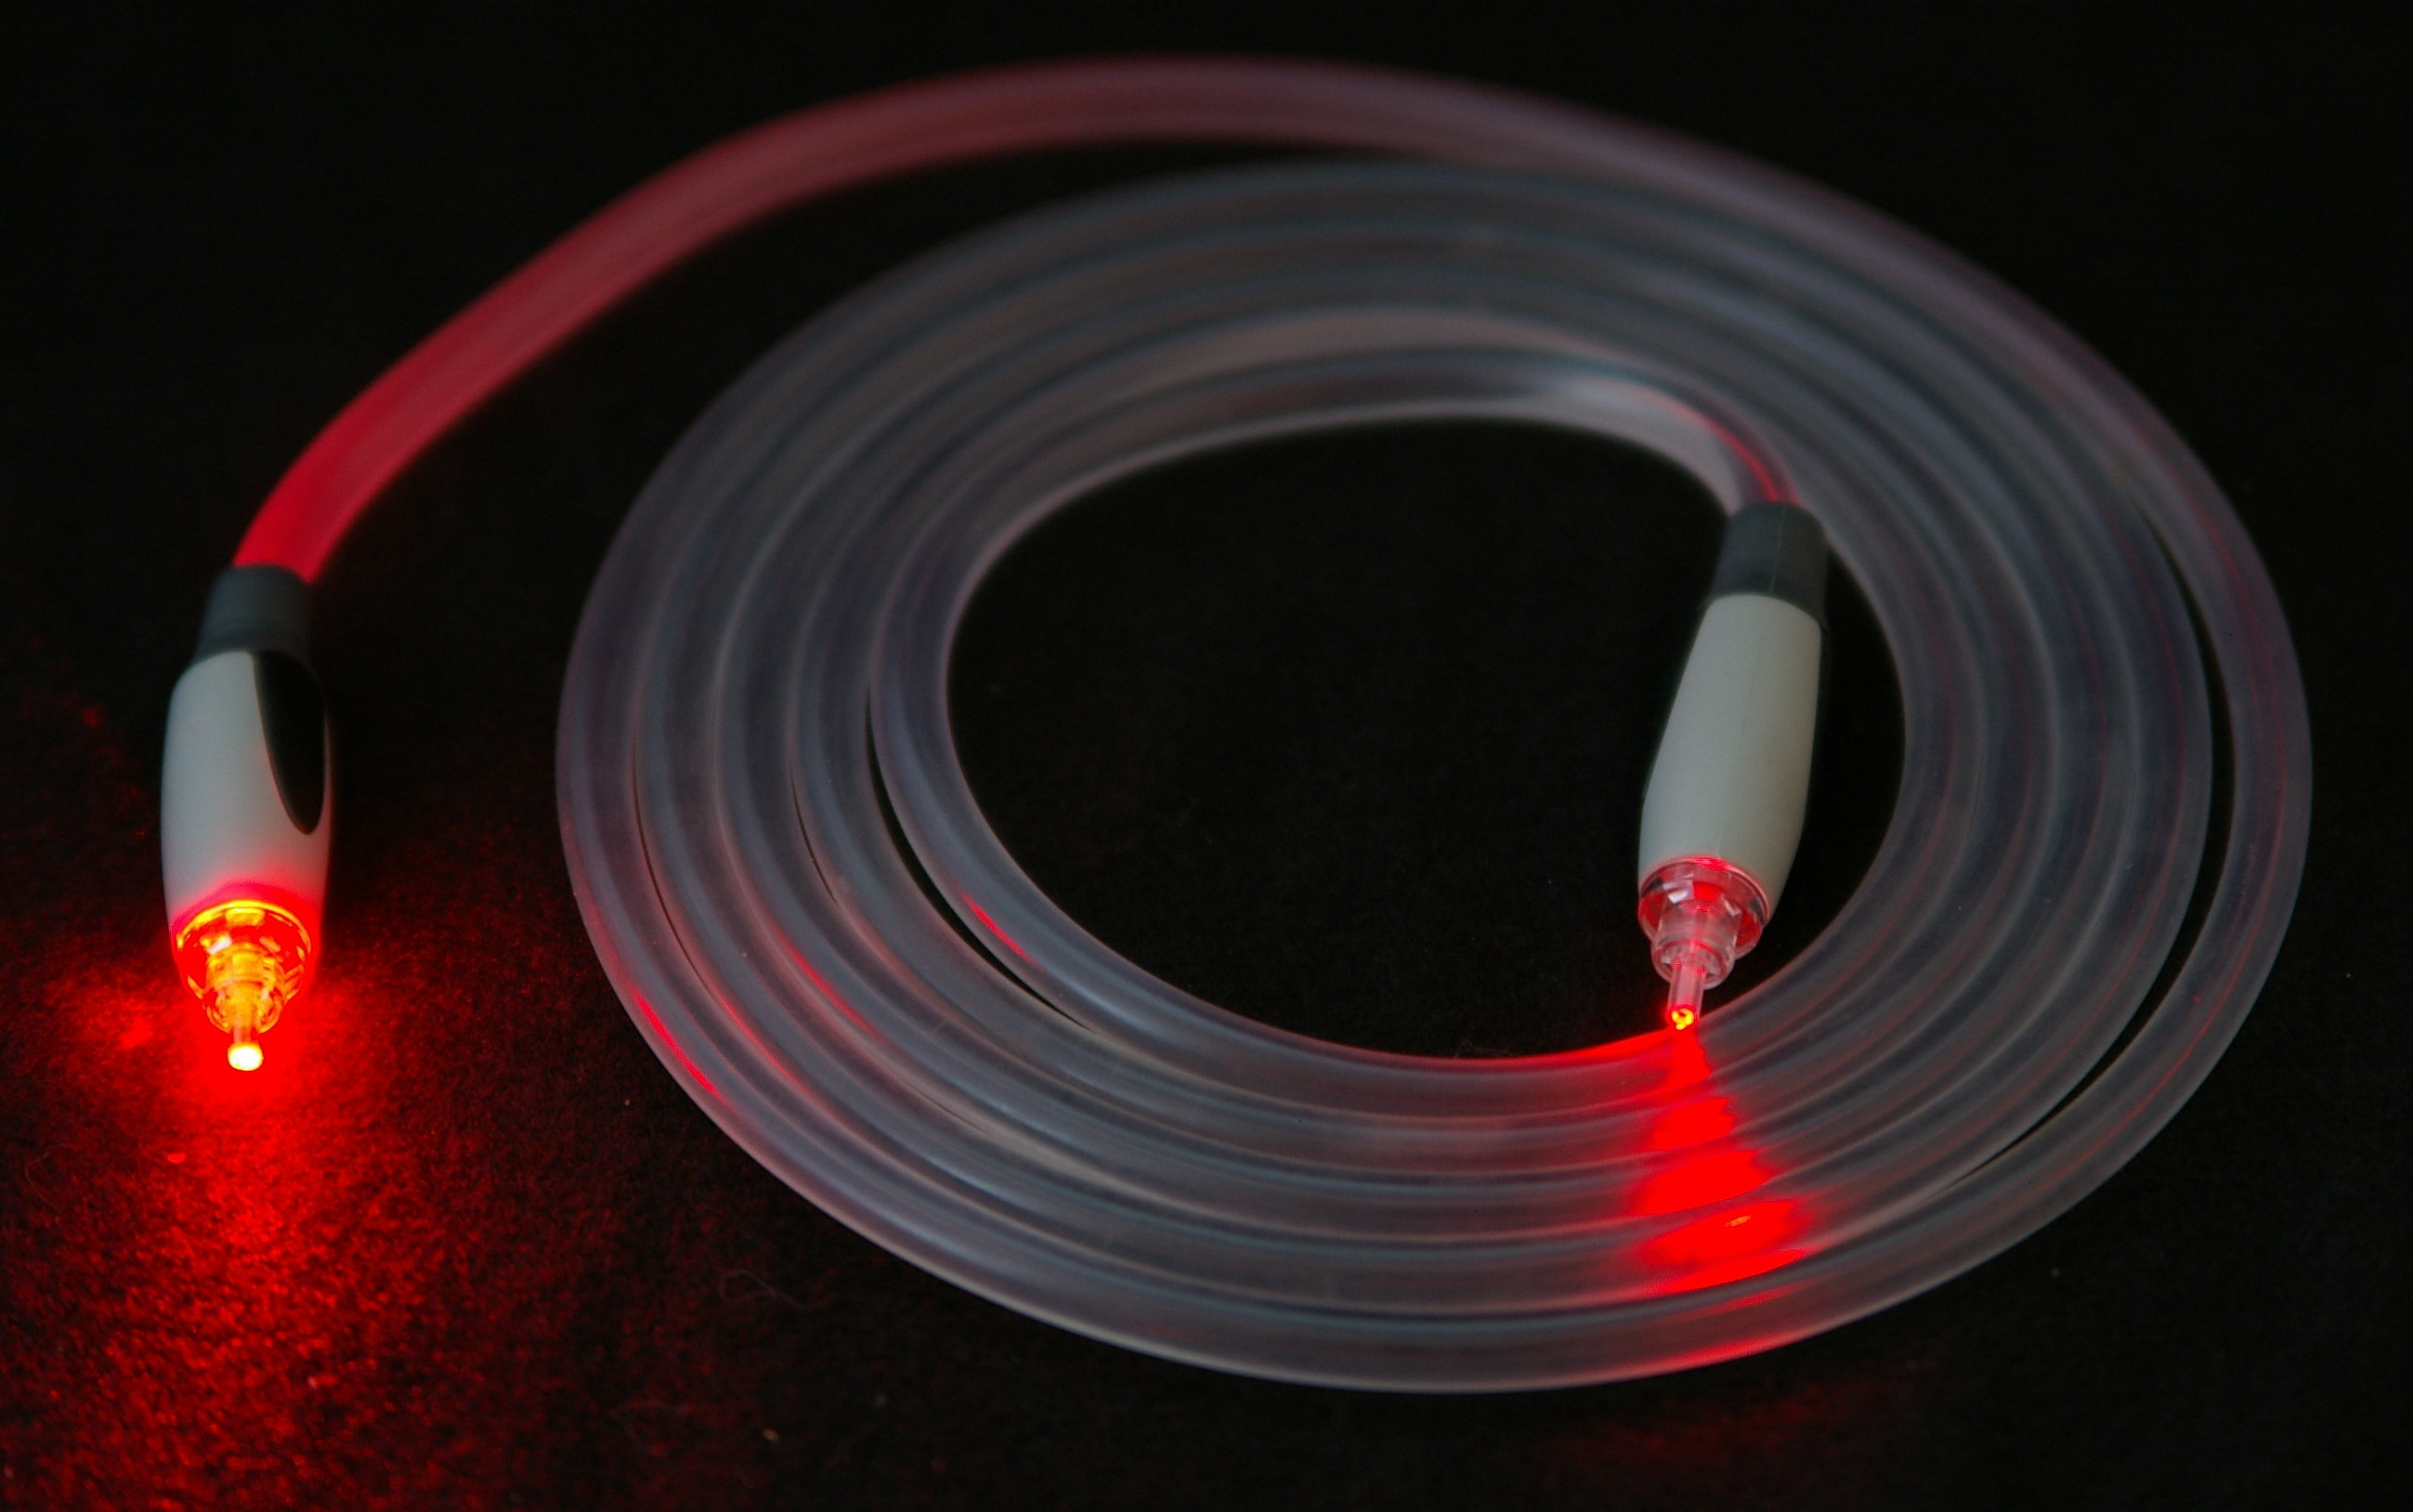
\includegraphics[width=4.3cm]{../physical/Fiber_optic_illuminated.jpeg}
}; \&
\node[draw,label={[credit]south:Dmitry G, CC BY-SA 3.0, via Wikimedia Commons},
      label={[type]north:bundle of wires}] (eth)  {
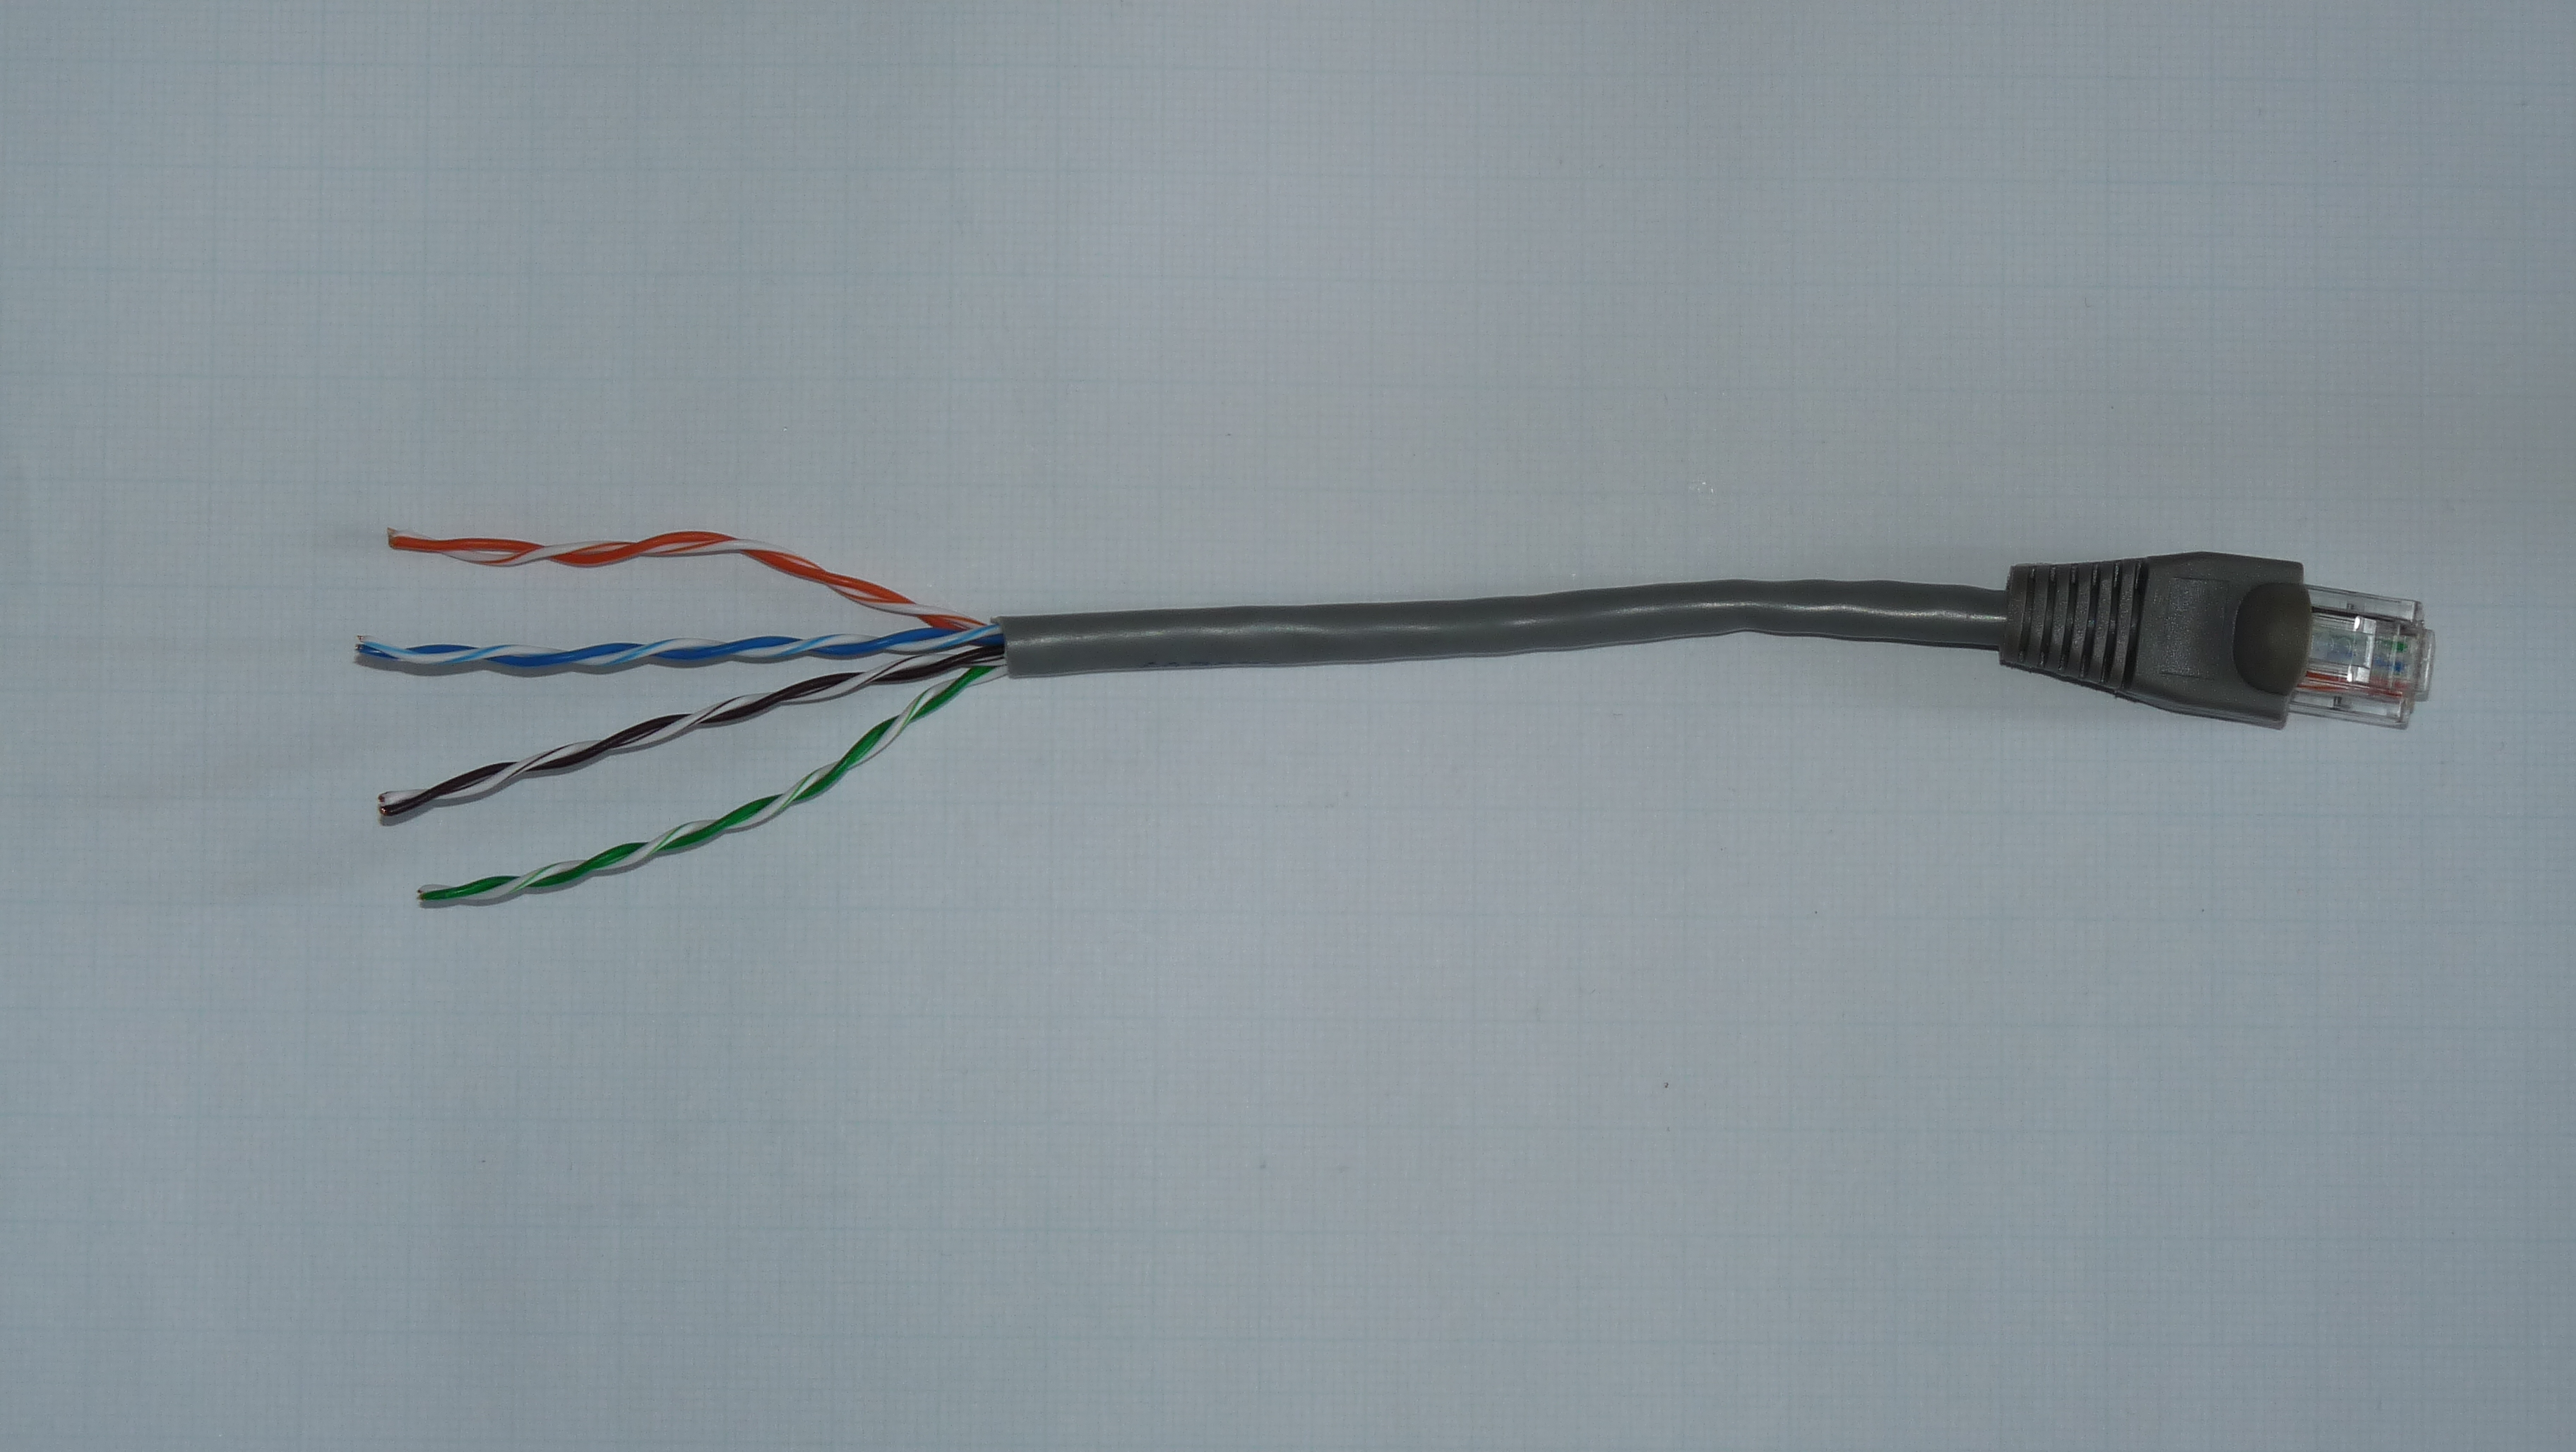
\includegraphics[width=4.3cm]{../physical/Ethernet_cable.jpeg}
}; \&
\node[draw,label={[credit]south:Adamantios, CC BY-SA 3.0, via Wikimedia Commons},
      label={[type]north:infrared through air}] (fso)  {
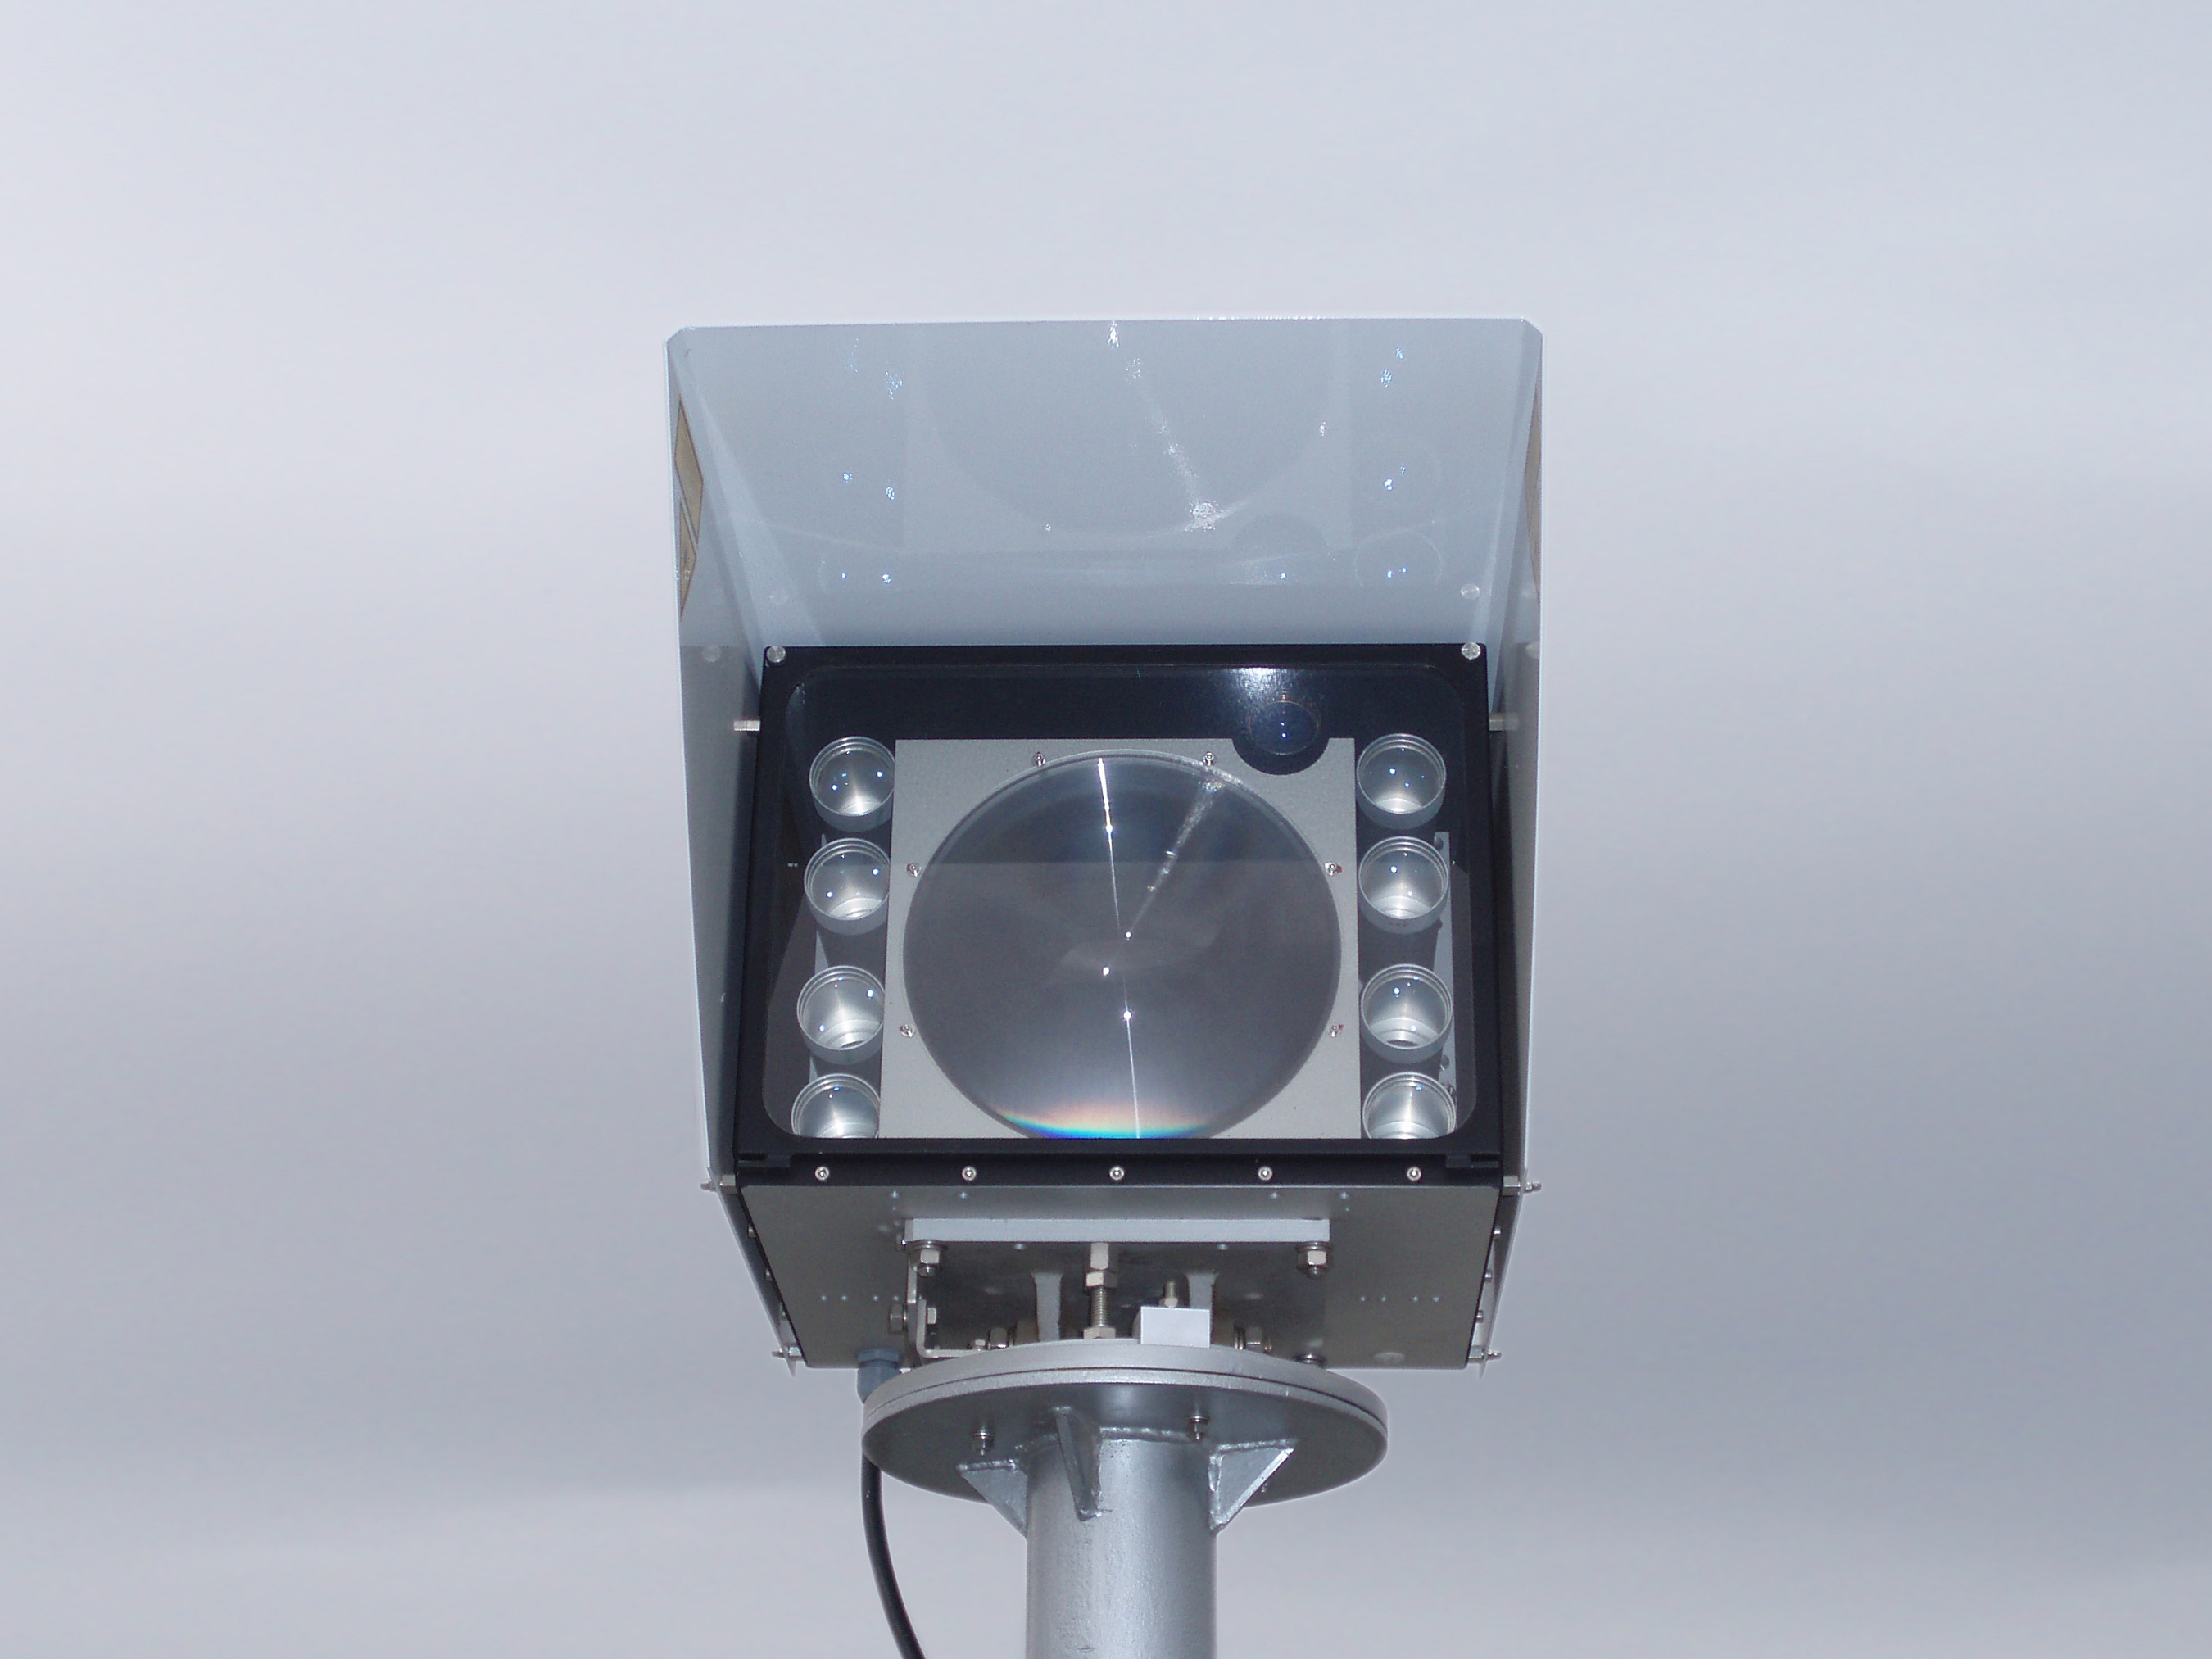
\includegraphics[width=3.7cm]{../physical/FSO-gigabit-laser-link-0a.jpeg}
}; \\
\node[draw,label={[credit]south:FDominec, CC BY-SA 3.0, via Wikimedia Commons},
      label={[type]north:single wire}] (coax)  {
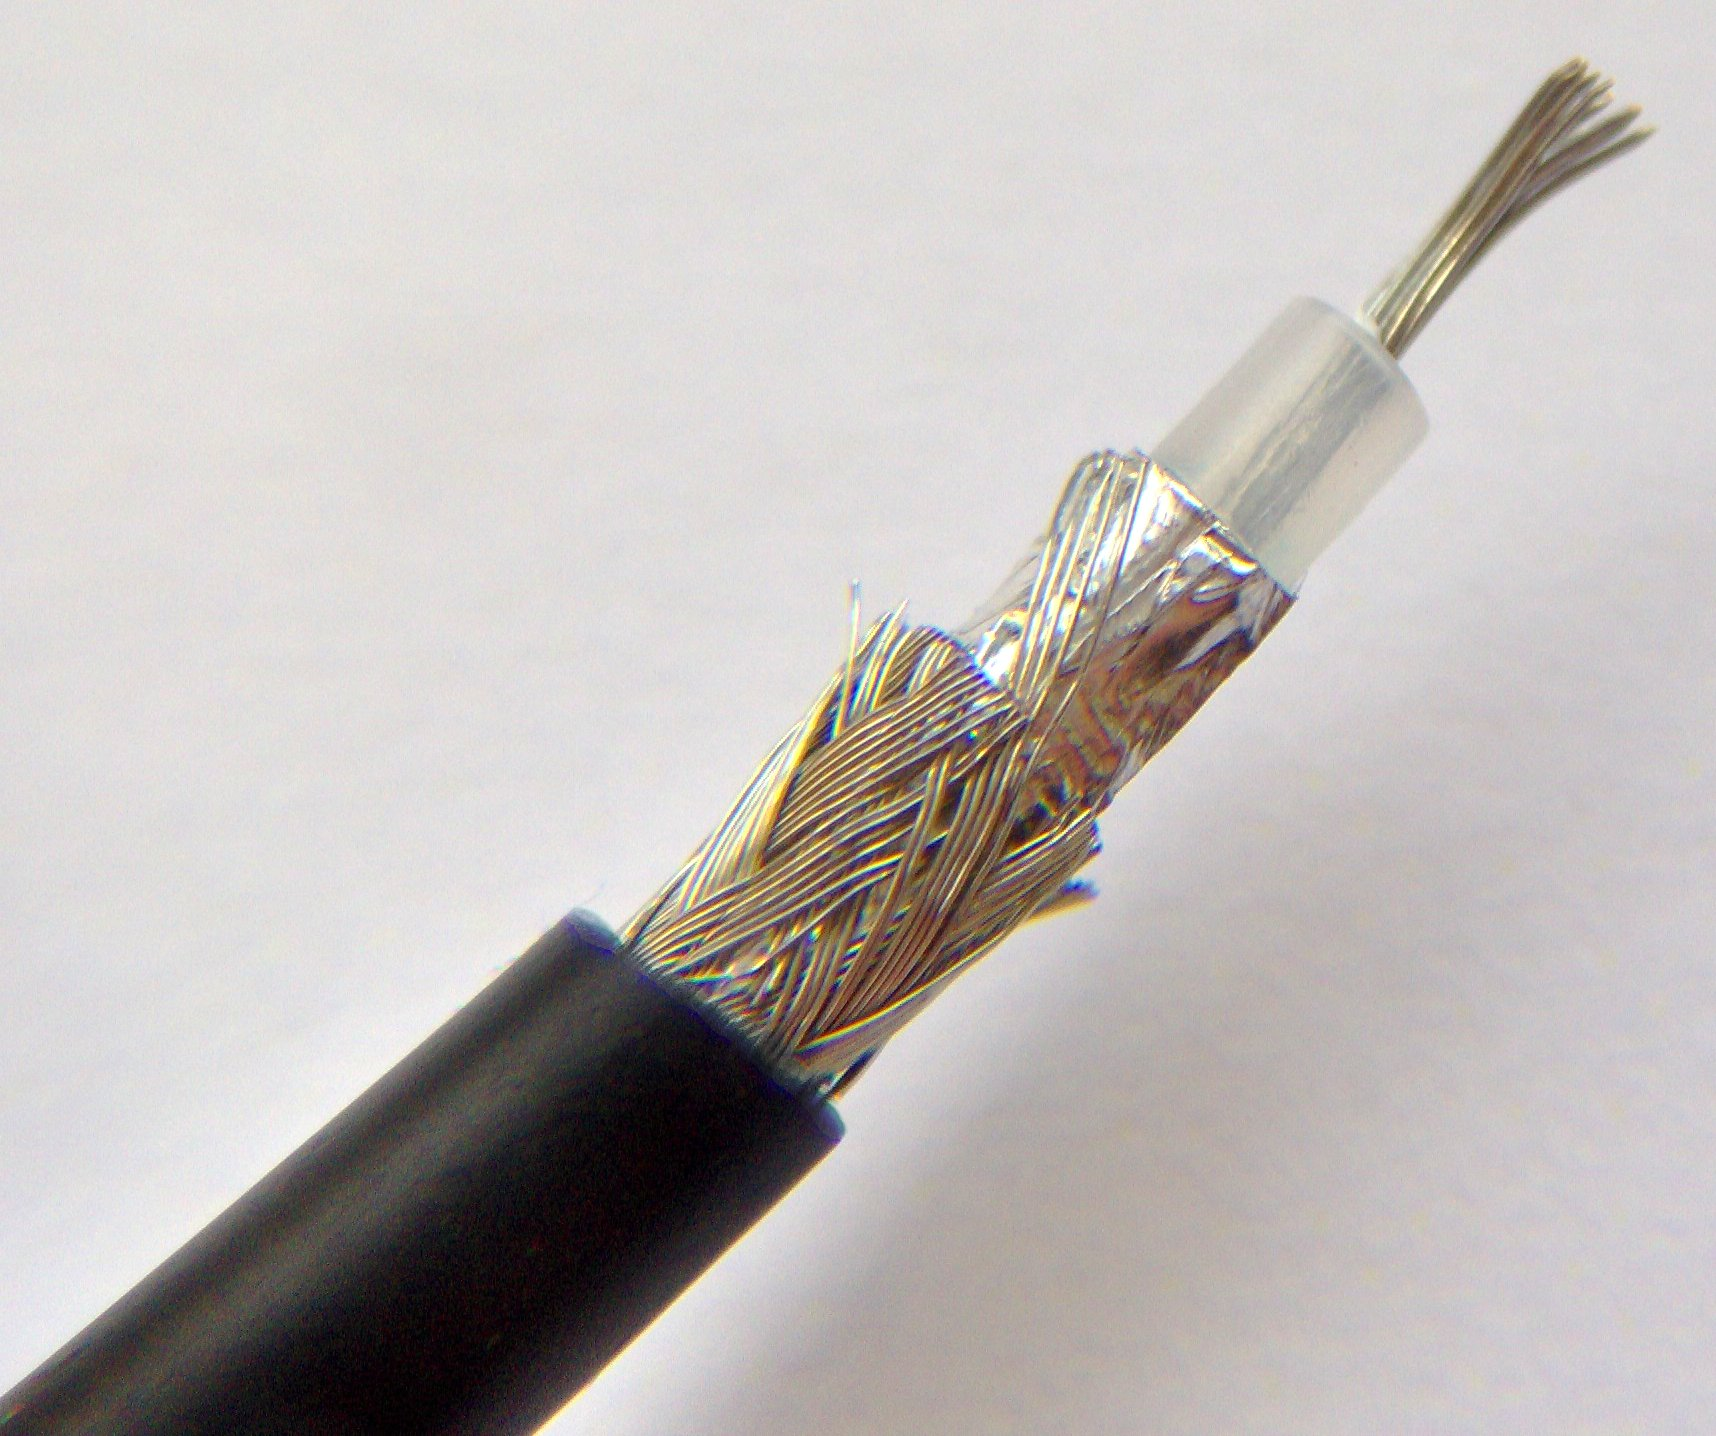
\includegraphics[width=3.3cm]{../physical/Coaxial_cable_cut.jpeg}
}; \&
\node[draw,label={[credit]south:Evan-Amos, via Wikimedia Commons},
      label={[type]north:radio}] (wifi)  {
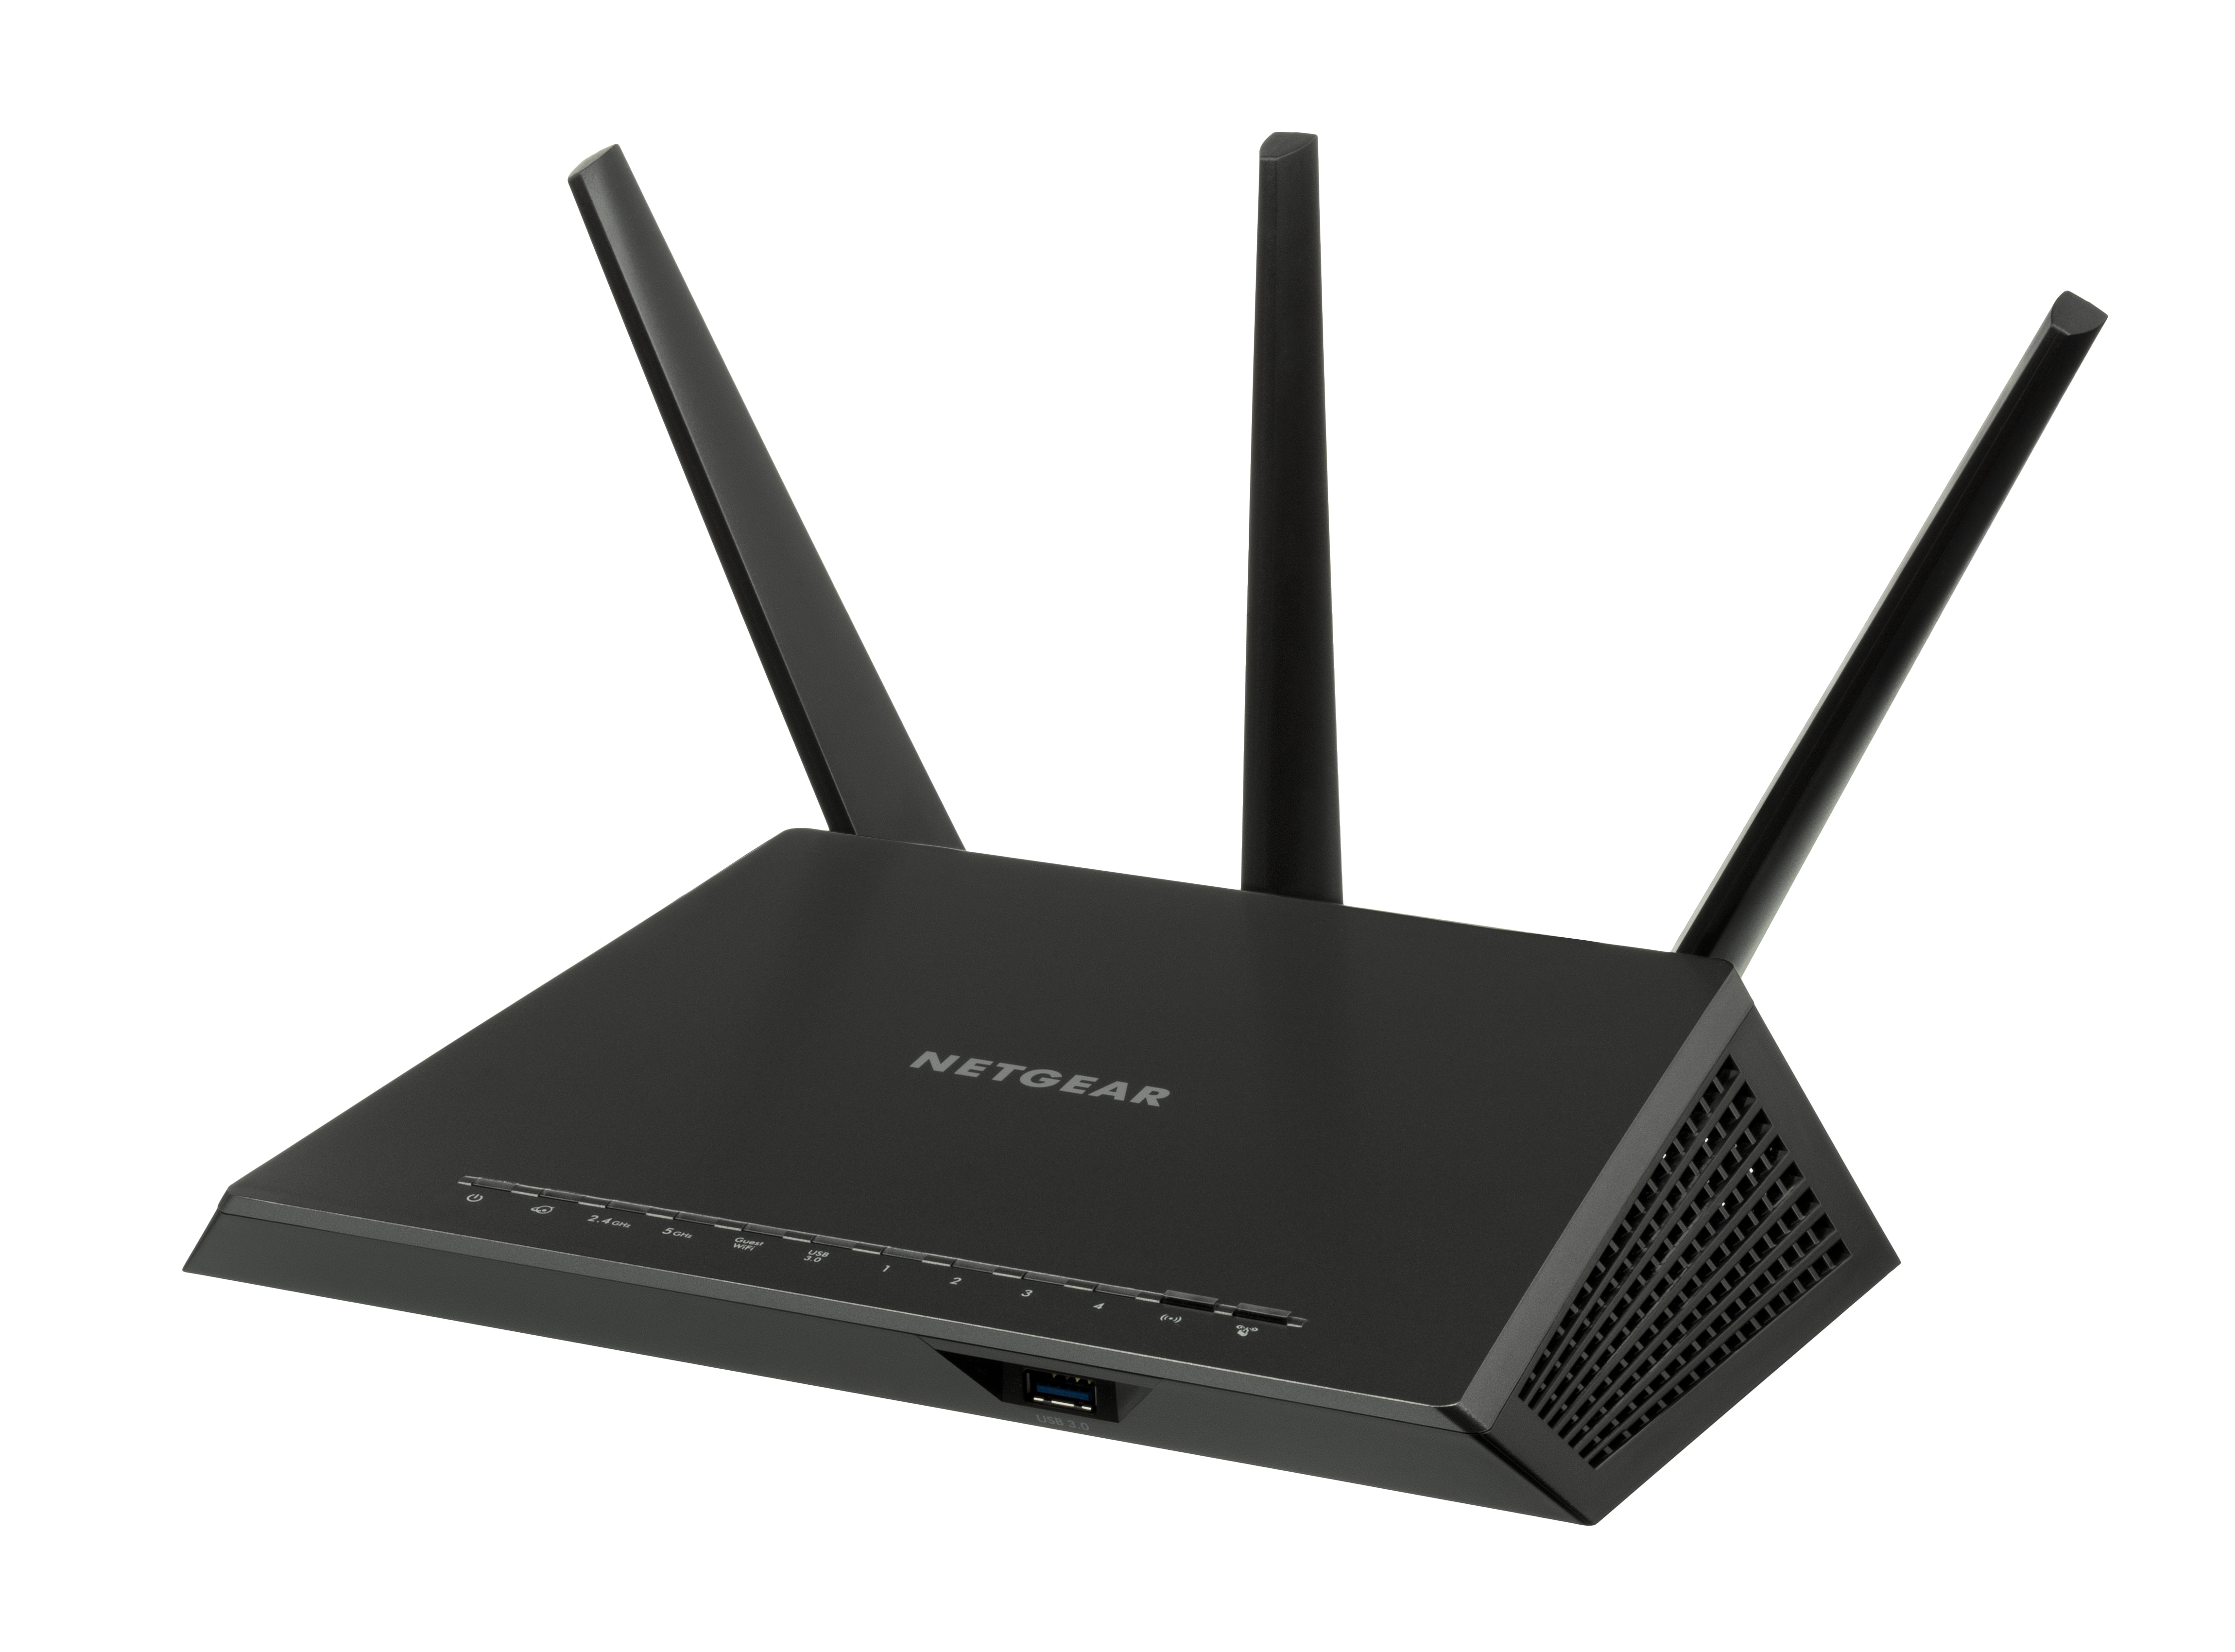
\includegraphics[width=3.7cm]{../physical/Netgear-Nighthawk-AC1900-WiFi-Router.jpeg}
}; \& \node[draw=none] (dotdot place) {}; \\
};
\node[draw=none,font=\Huge,anchor=center] (dotdot) at (wifi.east -| dotdot place.center){\ldots};
\end{tikzpicture}
\end{frame}


\subsection{transmitting a signal}
\usetikzlibrary{arrows.meta,calc,fadings,patterns}
\begin{frame}{transmitting a signal}
    \begin{itemize}
    \item can vary\ldots
        \begin{itemize}
        \item voltage
        \item radio/light intensity 
        \item radio/light frequency
        \item \ldots
        \end{itemize}
    \end{itemize}
\begin{tikzpicture}
\tikzset{
    axis/.style={draw,ultra thick,-Latex},
    signal/.style={draw,very thick,violet},
    axis label/.style={draw,thin,font=\small},
},
\begin{pgfonlayer}{fg}
    \draw[axis] (0, 0) -- (0, 3);
    \draw[axis] (0, 0) -- (14, 0);
\end{pgfonlayer}
\draw[axis label] (0, .3) -- ++ (-.2, 0) node[left] {low};
\draw[axis label] (0, 2.1) -- ++ (-.2, 0) node[left] {high};
\begin{scope}
    \clip (0, 0) rectangle (14, 3);
    %\begin{scope}[yshift=.3cm,y=1.8cm]
    %\draw[signal] (0, 0) -- (3, 0) -- (3, 1) -- (5, 1) -- (5, 0) -- (9, 0) -- (9, 1) -- (11, 1) -- (11, 0) -- (16, 0);
    %\end{scope}
    \begin{scope}[yshift=.3cm,y=0.6cm]
    \draw[signal] (0, 0) -- (3, 0) -- (3, 1) -- (5, 1) -- (5, 3) -- (9, 3) -- (9, 1) -- (11, 1) -- (11, 2) --
        (13, 2) -- (13, 0) -- (15, 0);
    \end{scope}
    \fill[white,path fading=west] (12, 0) rectangle (13.8, 3);
    \fill[white] (13.8, 0) rectangle (14, 3);
\end{scope}
\end{tikzpicture}
\end{frame}

\begin{frame}{some simplifying assumptions}
    \begin{itemize}
    \item signal low/high --- no in between
    \item only one `channel' 
        \begin{itemize}
        \item won't have multiple wires/antennas/frequencies/etc.
        \item won't modulate different things same time
        \end{itemize}
    \item want to send receive bits (0 or 1)
    \end{itemize}
\begin{tikzpicture}
\tikzset{
    axis/.style={draw,ultra thick,-Latex},
    signal/.style={draw,very thick,violet},
    axis label/.style={draw,thin,font=\small},
},
\begin{pgfonlayer}{fg}
    \draw[axis] (0, 0) -- (0, 3);
    \draw[axis] (0, 0) -- (14, 0);
\end{pgfonlayer}
\draw[axis label] (0, .3) -- ++ (-.2, 0) node[left] {low};
\draw[axis label] (0, 2.1) -- ++ (-.2, 0) node[left] {high};
\begin{scope}
    \clip (0, 0) rectangle (14, 3);
    \begin{scope}[yshift=.3cm,y=1.8cm]
    \draw[signal] (0, 0) -- (3, 0) -- (3, 1) -- (5, 1) -- (5, 0) -- (9, 0) -- (9, 1) -- (11, 1) -- (11, 0) -- (16, 0);
    \end{scope}
    \fill[white,path fading=west] (12, 0) rectangle (13.8, 3);
    \fill[white] (13.8, 0) rectangle (14, 3);
\end{scope}
\end{tikzpicture}
\end{frame}

\begin{frame}{clocking}
\begin{tikzpicture}
\tikzset{
    axis/.style={draw,ultra thick,-Latex},
    signal/.style={draw,very thick,violet},
    axis label/.style={draw,thin,font=\small},
    value/.style={font=\tt},
},
\begin{pgfonlayer}{fg}
    \draw[axis] (0, 0) -- (0, 3);
    \draw[axis] (0, 0) -- (14, 0);
\end{pgfonlayer}
\draw[axis label] (0, .3) -- ++ (-.2, 0) node[left] {low};
\draw[axis label] (0, 2.1) -- ++ (-.2, 0) node[left] {high};
\begin{scope}
    \clip (0, 0) rectangle (14, 3);
    \begin{scope}[yshift=.3cm,y=1.8cm]
    \draw[signal] (0, 0) -- (2.85, 0) -- (2.85, 1) -- (5.05, 1) -- (5.05, 0) -- (9.05, 0) -- (9.05, 1) -- (11.1, 1) -- (11.1, 0) -- (16, 0);
    \end{scope}
    \fill[white,path fading=west] (12, 0) rectangle (13.8, 3);
    \fill[white] (13.8, 0) rectangle (14, 3);
\end{scope}
\begin{visibleenv}<2,5>
\begin{scope}[yshift=-.8cm,xshift=1cm,x=2cm]
\foreach \x/\v in {0/0,1/1,2/0,3/0,4/1,5/0,6/0} {
    \draw[thick,dotted] (\x, -0.5) -- ++(0, 4.5cm);
    \node[value,anchor=north] at (\x+0.5, 0) {\v};
}
\end{scope}
\end{visibleenv}
\begin{visibleenv}<4,5>
\begin{scope}
\clip[overlay] (0, -10) rectangle (15, 10);
\begin{scope}[yshift=-.2cm,xshift=1.35cm,x=1.6cm]
\foreach \x/\v in {-1/0,0/0,1/1,2/0,3/0,4/0,5/1,6/0,7/0,8/0} {
    \draw[thick,dashed] (\x, -.5) -- ++(0, 4cm);
    \node[value,anchor=north] at (\x+0.5, 0) {\v};
}
\end{scope}
\end{scope}
\end{visibleenv}
\begin{visibleenv}<3,5>
\begin{scope}[yshift=-1.3cm,xshift=1cm,x=1cm]
\foreach \x/\v in {0/0,1/0,2/1,3/1,4/0,5/0,6/0,7/0,8/1,9/1,10/0,11/0} {
    \draw[thick,dashed] (\x, -.5) -- ++(0, 5cm);
    \node[value,anchor=north] at (\x+0.5, 0) {\v};
}
\end{scope}
\end{visibleenv}
\end{tikzpicture}
\end{frame}

\begin{frame}{keeping a clock}
\begin{tikzpicture}
\tikzset{
    axis/.style={draw,ultra thick,-Latex},
    signal/.style={draw,very thick,violet},
    axis label/.style={draw,thin,font=\small},
    value/.style={font=\tt},
},
\begin{pgfonlayer}{fg}
    \draw[axis] (0, 0) -- (0, 3);
    \draw[axis] (0, 0) -- (14, 0);
\end{pgfonlayer}
\draw[axis label] (0, .3) -- ++ (-.2, 0) node[left] {low};
\draw[axis label] (0, 2.1) -- ++ (-.2, 0) node[left] {high};
\begin{scope}
    \clip (0, 0) rectangle (14, 3);
    \begin{scope}[yshift=.3cm,y=1.8cm]
    \draw[signal] (0, 0) -- (2.85, 0) -- (2.85, 1) -- (5.05, 1) -- (5.05, 0) -- (9.05, 0) -- (9.05, 1) -- (11.1, 1) -- (11.1, 0) -- (16, 0);
    \end{scope}
    \fill[white,path fading=west] (12, 0) rectangle (13.8, 3);
    \fill[white] (13.8, 0) rectangle (14, 3);
\end{scope}

\begin{scope}[yshift=-4cm]
    \begin{pgfonlayer}{fg}
        \draw[axis] (0, 0) -- (0, 3);
        \draw[axis] (0, 0) -- (14, 0);
    \end{pgfonlayer}
    \draw[axis label] (0, .3) -- ++ (-.2, 0) node[left] {low};
    \draw[axis label] (0, 2.1) -- ++ (-.2, 0) node[left] {high};
    \begin{scope}
        \clip (0, 0) rectangle (14, 3);
        \begin{scope}[yshift=.3cm,y=1.8cm]
        \begin{visibleenv}<2->
        \draw[signal,alt=<3->{opacity=0.1}]
            (0, 1) -- (1, 1) -- (1, 0) -- (2, 0) -- (2, 1) 
        -- (2.95, 1) -- (2.95, 0) -- (4, 0) -- (4, 1) -- (5.08, 1) -- (5.08, 0)
        -- (6, 0) -- (6, 1) -- (7.05, 1) -- (7.05, 0) -- (8, 0) -- (8, 1)
        -- (8.95, 1) -- (8.95, 0) -- (10, 0) -- (10, 1) -- (11.0, 1) -- (11.0, 0)
        -- (12, 0) -- (12, 1) -- (13, 1) -- (13, 0) -- (14, 0) -- (14, 1) --(15, 1);
        \end{visibleenv}
        \begin{visibleenv}<3-4>
        \draw[signal]
            (0, 1) -- (1, 1) -- (1, 0) -- (2, 0) -- (2, 1) 
        -- (2.85, 1) edge[red] (2.85, 0) (2.85,0) -- (3.9, 0) edge[red] (3.9, 1) (3.9, 1)-- (5.05, 1) edge[red] (5.05, 0)
        (5.05, 0)
        -- (6, 0) -- (6, 1) -- (7.05, 1) -- (7.05, 0) -- (8, 0) -- (8, 1)
        -- (9.05, 1) edge[red] (9.05, 0) (9.05, 0) -- (10.05, 0) edge[red] (10.05, 1) (10.05, 1) -- (11.1, 1) edge[red] (11.1, 0) (11.0, 0)
        -- (12, 0) -- (12, 1) -- (13.1, 1) edge[red] (13.1, 0) (13.1, 0) -- (14, 0) -- (14, 1) --(15, 1);
        \end{visibleenv}
        \end{scope}
        \fill[white,path fading=west] (12, 0) rectangle (13.8, 3);
        \fill[white] (13.8, 0) rectangle (14, 3);
    \end{scope}
\end{scope}
\begin{visibleenv}<2->
    \begin{scope}[yshift=-.2cm,xshift=1cm,x=2cm]
    \foreach \x/\v in {0/0,1/1,2/0,3/0,4/1,5/0,6/0} {
        \node[value,anchor=north] at (\x+0.5, 0) {\v};
    }
    \end{scope}
    \begin{scope}[yshift=-.2cm]
    \foreach \loc in {1,2.95,5.08,7.05,8.95,11,13,15} {
        \draw[thick,dashed] (\loc, -4) -- ++(0, 7);
    }
    \end{scope}
\end{visibleenv}
\begin{visibleenv}<3-4>
    \begin{scope}[yshift=-.2cm]
    \tikzset{
        marked/.style={red,ultra thick},
    }
    \foreach \loc/\mark in {1/,2.85/marked,5.05/marked,7.05/,9.05/marked,11.1/marked,13.1/marked,15.1/} {
        \draw[thick,dashed,\mark] (\loc, -4) -- ++(0, 7);
    }
    \end{scope}
\end{visibleenv}
\end{tikzpicture}
\end{frame}

\begin{frame}{self-synchronizing?}
    \begin{itemize}
    \item can resynchronize clock by looking for transitions
    \item but doesn't work if lots of consecutive 0s or 1s
    \vspace{.5cm}
    \item also, need to know where low and high point is
    \item important to have transitions to low/high to calibrate this
    \end{itemize}
\end{frame}

\begin{frame}{Manchester encoding}
\begin{tikzpicture}
\node (fig) { 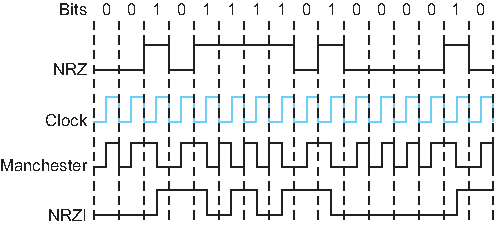
\includegraphics[width=0.9\textwidth]{../physical/SysApproach-2-Fig-25.pdf} };
\end{tikzpicture}
\imagecredit{Figure 25 from Section 2.2 of \textit{Computer Networks: A Systems Approach} (6th ed) (Peterson and Davie)}
\end{frame}

\begin{frame}{problem with Manchester}
    \begin{itemize}
    \item fixed the problem of too few transitions
    \vspace{.5cm}
    \item but now most transitions don't send information
    \item means we aren't making goo duse of wire/etc. capacity
    \vspace{.5cm}
    \item there are more clever compromises
        \begin{itemize}
        \item (example: 4B5B encoding)
    \end{itemize}
\end{frame}

\begin{frame}{other better encoding options}
    \begin{itemize}
    \item vary more than just one thing
        \begin{itemize}
        \item example: pulse amplitude and duration
        \end{itemize}
    \item use more than just low/high
    \item \ldots much more
    \vspace{.5cm}
    \item probably covered in ECE Signals course?
    \end{itemize}
\end{frame}


\subsection{synchronizing (short)}


\begin{frame}{self-synchronizing?}
    \begin{itemize}
    \item can resynchronize clock by looking for transitions
    \item but doesn't work if lots of consecutive 0s or 1s
    \vspace{.5cm}
    \item also, need to know where low and high point is
    \item important to have transitions to low/high to calibrate this
    \end{itemize}
\end{frame}

\begin{frame}{self-sync and `start-message'}
    \begin{itemize}
    \item one idea: set start-message to have lots of 0/1/0/1/0/1/0/1/etc.
        \begin{itemize}
        \item something 10Mbit Ethernet does
        \end{itemize}
    \item but probably not enough to ensure things stay in sync on big message
    \vspace{.5cm}
    \item alternate strategy --- use encoding that adds extra transitions
    \item example: Manchester encoding
    \end{itemize}
\end{frame}


\subsectoin{better options?}
\begin{frame}{other better encoding options}
    \begin{itemize}
    \item vary more than just one thing
        \begin{itemize}
        \item example: pulse amplitude and duration
        \end{itemize}
    \item use more than just low/high
    \item \ldots much more
    \vspace{.5cm}
    \item probably covered in ECE Signals course?
    \end{itemize}
\end{frame}




\section{framing}

\subsection{aligning the bits}

\usetikzlibrary{fit,matrix}
\begin{frame}{aligning bits}
    \begin{itemize}
    \item let's transmit these (binary) messages:
        \begin{itemize}
        \item \tt 001
        \item \tt 0110
        \item \tt 0010
        \end{itemize}
    \end{itemize}
\begin{tikzpicture}
\matrix[tight matrix no line,nodes={text width=.35cm,font=\large\tt}] (msg) {
|[alias=s1]| 0 \& 0 \& |[alias=e1]| 1 \& |[alias=s2]| 0 \& 1 \& 1 \& |[alias=e2]| 0 \& 
|[alias=s3]| 0 \& 0 \& 1 \& |[alias=e3]| 0 \\
};
\foreach \x in {1,2,3} {
    \node[inner sep=0mm,outer sep=0mm,draw,red,very thick,fit=(s\x) (e\x),alt=<2>{opacity=0.1}] {};
}
\end{tikzpicture}
\begin{itemize}
\item<2-> problem: can't tell where messages/start end
\end{itemize}
\end{frame}


\subsection{size strategy}

\usetikzlibrary{decorations.pathreplacing}
\begin{frame}{size `header'}
\begin{itemize}
    \item let's transmit these (binary) messages:
        \begin{itemize}
        \item \tt 001
        \item \tt 0110
        \item \tt 0010
        \end{itemize}
    \item put 3-bit message size at beginning of messages
\end{itemize}
\begin{tikzpicture}
\matrix[tight matrix no line,nodes={text width=.35cm,font=\large\tt}] (msg) {
|[alias=h1]| 0 \& 1 \& 1 \& |[alias=s1]| 0 \& 0 \& |[alias=e1]| 1 \& 
|[alias=h2]| 1 \& 0 \& 0 \& |[alias=s2]| 0 \& 1 \& 1 \& |[alias=e2]| 0 \& 
|[alias=h3]| 1 \& 0 \& 0 \& |[alias=s3]| 0 \& 0 \& 1 \& |[alias=e3]| 0 \\
};
\foreach \x in {1,2,3} {
    \node[inner sep=0mm,outer sep=0mm,draw,green,very thick,fit=(s\x) (e\x)] {};
    \node[inner sep=0mm,outer sep=0mm,fill=blue,fill opacity=0.1,very thick,fit=(h\x) (s\x.west)] {};
    \draw[very thick,decorate,decoration={brace,mirror}] 
        ([xshift=.1cm,yshift=-.1cm]h\x.south west) -- ([xshift=-.1cm,yshift=-.1cm]e\x.south east) {};
}
\end{tikzpicture}
\begin{itemize}
\item read header, then determine number of bits to read before next header
\item<2-> assumption: \myemph<2>{no gaps between messages?}
    \begin{itemize}
    \item need to transmit \textit{something} in between messages
    \end{itemize}
\end{itemize}
\end{frame}



\subsection{start/end symbol strategy}

\begin{frame}{start/end symbol}
    \begin{itemize}
    \item alternate idea: use bit sequence to mark beginning/end
    \item example choice: send 010 between each frame
    \item send extra 010s when no frames to send
    \end{itemize}
\begin{tikzpicture}
\matrix[tight matrix no line,nodes={text width=.35cm,font=\large\tt}] (msg) {
|[alias=h1]| 0 \& 1 \& 0 \& |[alias=s1]| 0 \& |[alias=bform1s]| 0 \& |[alias=e1,alias=bform1e]| 1 \& 
|[alias=h2]| 0 \& 1 \& 0 \& |[alias=s2,alias=bform2s]| 0 \& |[alias=bform2e]| 1 \& 1 \& |[alias=e2]| 0  \&
|[alias=h3]| 0 \& 1 \& 0 \& |[alias=s3]| 0 \& |[alias=false start,alias=bform3s]| 0 \& |[alias=bform3e]| 1 \& |[alias=e3,alias=false end]| 0 \& |[alias=h4]| 0 \& 1 \& 0 \& |[alias=s4]| ~ \\
};
\foreach \x in {1,2,3} {
    \node[inner sep=0mm,outer sep=0mm,draw,green,alt=<2>{opacity=0.1},very thick,fit=(s\x) (e\x)] {};
}
\foreach \x in {1,2,3,4} {
    \node[inner sep=0mm,outer sep=0mm,fill=blue,fill opacity=0.1,alt=<3>{fill opacity=0.05},very thick,fit=(h\x) (s\x.west)] {};
}
\foreach \x in {1,2,3} {
    \draw[very thick,decorate,decoration={brace,mirror}] 
        ([xshift=.1cm,yshift=-.1cm]s\x.south west) -- ([xshift=-.1cm,yshift=-.1cm]e\x.south east) {};
    \begin{visibleenv}<3>
    \fill[fill opacity=0.1,red,draw=violet,ultra thick,dotted] (bform\x s.south west) rectangle (bform\x e.north east);
    \end{visibleenv}
}
\begin{visibleenv}<2>
\node[draw=red,ultra thick,fit=(false start) (false end),inner sep=1mm,outer sep=0mm] {};
\end{visibleenv}
\end{tikzpicture}
\begin{itemize}
\item<2-> problem: \myemph<2>{messages can contain \texttt{010} or end with \texttt{01}}
\item<3-> one solution: replace \texttt{01} in messages with \texttt{011}
    \begin{itemize}
    \item (need to undo replacement when receiving)
    \end{itemize}
\end{itemize}
\begin{visibleenv}<3->
\begin{tikzpicture}
\matrix[tight matrix no line,nodes={text width=.35cm,font=\large\tt}] (msg) {
|[alias=h1]| 0 \& 1 \& 0 \& |[alias=s1]| 0 \& |[alias=xform1s]| 0 \& 1 \& |[alias=xform1e,alias=e1]| 1 \&  
|[alias=h2]| 0 \& 1 \& 0 \& |[alias=s2,alias=xform2s]| 0 \& 1 \& |[alias=xform2e]| 1 \& 1 \& |[alias=e2]| 0 \&
|[alias=h3]| 0 \& 1 \& 0 \& |[alias=s3]| 0 \&|[alias=xform3s]| 0 \& 1 \& |[alias=xform3e,alias=e3]| 1 \& |[alias=e3]| 0 \& |[alias=h4]| 0 \& 1 \& 0 \& |[alias=s4]| ~ \\
};
\foreach \x in {1,2,3} {
    \node[inner sep=0mm,outer sep=0mm,draw,green,alt=<2>{opacity=0.1},very thick,fit=(s\x) (e\x)] {};
}
\foreach \x in {1,2,3,4} {
    \node[inner sep=0mm,outer sep=0mm,fill=blue,fill opacity=0.1,alt=<3>{fill opacity=0.05},very thick,fit=(h\x) (s\x.west)] {};
}
\foreach \x in {1,2,3} {
    \draw[very thick,decorate,decoration={brace,mirror}] 
        ([xshift=.1cm,yshift=-.1cm]s\x.south west) -- ([xshift=-.1cm,yshift=-.1cm]e\x.south east) {};
    \fill[fill opacity=0.1,red,draw=violet,ultra thick,dotted] (xform\x s.south west) rectangle (xform\x e.north east);
}
\end{tikzpicture}
\end{visibleenv}
\end{frame}

\begin{frame}[fragile]{escaping?}
    \begin{itemize}
    \item can think of replacement similar to escaping strings in C
        \begin{itemize}
        \item start/end marker is \verb|"|
        \item \verb|"| $\rightarrow$ \verb|\"|
        \item \verb|\| $\rightarrow$ \verb|\\|
        \end{itemize}
    \item represent \verb|foo \R"3"13\| using \verb|"foo \\R\"3\"13\\"|
    \item but needed tweaks to idea to work with bits instead of bytes
    \vspace{.5cm}
    \item<2-> some physical layers allow transmitting bytes at a time
    \item<2-> example: upcoming assignment
    \item<2-> framing protocols for those (example: PPP) use \textbackslash-like idea
    \end{itemize}
\end{frame}

\begin{frame}{help from physical layer?}
    \begin{itemize}
    \item suppose instead of transmitting 0 or 1
    \item \ldots physical layer transmits 0 or 1 or 2 or 3 or 4
    \item probably going to `waste' one of these values
        \begin{itemize}
        \item example: transmit every two bits as 0 or 1 or 2 or 3
        \end{itemize}
    \vspace{.5cm}
    \item<2-> idea: take advantage of leftover `symbol' 4
    \item<2-> use it to send start/end
        \begin{itemize}
        \item similar idea used in many versions of Ethernet
        \end{itemize}
    \end{itemize}
\end{frame}


\subsection{aside: start/end ambiguity}
\begin{frame}{bad choice of start/end (1)}
    \begin{itemize}
    \item [this slide added 6 Sep 2024]
    \item let's say we choose delimiter \texttt{0000}
    \item what do we need to escape?
    \end{itemize}
\begin{tabular}{l}
A. any 0000 \\
A. any 000 \\
B. any 00 \\
C. any 0 \\
\end{tabular}
\end{frame}

\begin{frame}{bad choice of start/end (1)}
    \begin{itemize}
    \item sending \texttt{10} and \texttt{01}
        \begin{itemize}
        \item {\tt \myemph{10}0000\myemph{01}0000}
        \end{itemize}
    \item sending \texttt{1} and \texttt{001}
        \begin{itemize}
        \item {\tt \myemph{1}0000\myemph{001}0000}
        \end{itemize}
    \vspace{.5cm}
    \item oops!
    \item textbook example: start/end = {\tt 01111110}
    \end{itemize}
\end{frame}



\subsection{types of transmission errors}

% FIXME: worth keeping?
\begin{frame}<1>[label=transmitErrorType]{types of transmission errors}
    \begin{itemize}
    \item \myemph<2>{desynchronization}:
        \begin{itemize}
        \item missing bits/bytes
        \item adding bits/bytes
        \end{itemize}
    \item \myemph<3>{flipping bits}
        \begin{itemize}
        \item from `noise'/`interference'
        \end{itemize}
    \end{itemize}
\end{frame}

\againframe<2>{transmitErrorType}

\begin{frame}{desynchronization and framing (1)} 
    \begin{itemize}
    \item with purely size-based framing 
        \begin{itemize}
        \item almost all future sizes messed up
        \end{itemize}
    \end{itemize}
\begin{tikzpicture}
\tikzset{
    disappears/.style={opacity=0.1},
}
\matrix[tight matrix no line,nodes={text width=.35cm,font=\large\tt,name prefix=norm-}] (msg) {
|[alias=h1]| 0 \& 1 \& 1 \& |[alias=s1]| 0 \& 1 \& |[alias=e1]| 0 \& 
|[alias=h2]| 1 \& 0 \& 0 \& |[alias=s2]| 0 \& 1 \& 1 \& |[alias=e2]| 0 \& 
|[alias=h3]| 1 \& 0 \& 0 \& |[alias=s3]| 0 \& 1 \& 1 \& |[alias=e3]| 1 \& \ldots \& ~ \& \ldots \\
};
\matrix[anchor=north west,tight matrix no line,nodes={text width=.35cm,font=\large\tt,name prefix=bad-}] (msg alt)
at ([yshift=-1cm]msg.south west) {
|[disappears]| \sout{0} \& |[alias=h1]| 1 \& 1 \& 0 \& |[alias=s1]| 1 \& 0 \& 
1 \& 0 \& 0 \& |[alias=e1]| 0 \& |[alias=h2]| 1 \& 1 \& 0 \& 
|[alias=s2]| 1 \& 0 \& 0 \& 0 \& 1 \& |[alias=e2]| 1 \& |[alias=h3]| 1 \& |[alias=s3]| \ldots \& |[alias=e3]| ~ \& \ldots \\
};
\foreach \x in {1,2,3} {
    \foreach \pfx in {norm,bad} {
        \node[inner sep=0mm,outer sep=0mm,draw,green,very thick,fit=(\pfx-s\x) (\pfx-e\x)] {};
        \node[inner sep=0mm,outer sep=0mm,fill=blue,fill opacity=0.1,very thick,fit=(\pfx-h\x) (\pfx-s\x.west)] {};
        \draw[very thick,decorate,decoration={brace,mirror}] 
            ([xshift=.1cm,yshift=-.1cm]\pfx-h\x.south west) -- ([xshift=-.1cm,yshift=-.1cm]\pfx-e\x.south east) {};
    }
}
\end{tikzpicture}
\end{frame}

\begin{frame}{desynchronization and framing (2)}
\begin{itemize}
\item with start/end marker idea
    \begin{itemize}
    \item can have start/end-marker corrupted or added by corruption
    \item may mess up multiple frames, but will eventually be resync'd
    \end{itemize}
\end{itemize}
\begin{tikzpicture}
\tikzset{
    disappears/.style={opacity=0.1},
}
\matrix[tight matrix no line,nodes={text width=.35cm,font=\large\tt,name prefix=norm-}] (msg norm) {
|[alias=h1]| 0 \& 1 \& 0 \& |[alias=s1]| 0 \& |[alias=xform1s]| 0 \& 1 \& |[alias=xform1e,alias=e1]| 1 \&  
|[alias=h2]| 0 \& 1 \& 0 \& |[alias=s2,alias=xform2s]| 0 \& 1 \& |[alias=xform2e]| 1 \& 1 \& |[alias=e2]| 0 \&
|[alias=h3]| 0 \& 1 \& 0 \& |[alias=s3]| 0 \&|[alias=xform3s]| 0 \& 1 \& |[alias=xform3e,alias=e3]| 1 \& |[alias=e3]| 0 \& |[alias=h4]| 0 \& 1 \& 0 \& |[alias=s4]| ~ \\
};
\matrix[tight matrix no line,nodes={text width=.35cm,font=\large\tt,name prefix=bad-},
    anchor=north west] (msg bad) at ([yshift=-1cm]msg norm.south west) {
|[alias=h1]| 0 \& 1 \& 0 \& |[alias=s1]| 0 \& |[alias=xform1s]| 0 \& 1 \& |[alias=xform1e,alias=e1]| 1 \&  
|[]| 0 \& |[disappears]| \sout{1} \& 0 \& |[alias=xform2s]| 0 \& 1 \& |[alias=xform2e]| 1 \& 1 \& |[alias=e1]| 0 \&
|[alias=h2]| 0 \& 1 \& 0 \& |[alias=s2]| 0 \&|[alias=xform3s]| 0 \& 1 \& |[alias=xform3e,alias=e3]| 1 \& |[alias=e2]| 0 \& |[alias=h3]| 0 \& 1 \& 0 \& |[alias=s3]| ~ \\
};
\foreach \pfx/\maxM/\maxH/\maxS in {norm/3/4/3,bad/2/3/3} {
    \foreach \x in {1,...,\maxM} {
        \node[inner sep=0mm,outer sep=0mm,draw,green,very thick,fit=(\pfx-s\x) (\pfx-e\x)] {};
        \draw[very thick,decorate,decoration={brace,mirror}] 
            ([xshift=.1cm,yshift=-.1cm]\pfx-s\x.south west) -- ([xshift=-.1cm,yshift=-.1cm]\pfx-e\x.south east) {};
    }
    \foreach \x in {1,...,\maxH} {
        \node[inner sep=0mm,outer sep=0mm,fill=blue,fill opacity=0.1,very thick,fit=(\pfx-h\x) (\pfx-s\x.west)] {};
    }
    \foreach \x in {1,...,\maxS} {
        \fill[fill opacity=0.1,red,draw=violet,ultra thick,dotted] (\pfx-xform\x s.south west) rectangle (\pfx-xform\x e.north east);
    }
}
\end{tikzpicture}
\end{frame}

\begin{frame}{fixed-sized frames}
    \begin{itemize}
    \item suppose all packets are same size
    \item ``clock-based framing''
    \item example: SONET looks for start symbol every 810 bytes
        \begin{itemize}
        \item if starts being missing, try to resync
        \end{itemize}
    \end{itemize}
\end{frame}

\againframe<3>{transmitErrorType}

\begin{frame}{flipping bits?}
    \begin{itemize}
    \item flipping bits basically has same problems as synchornization
        \begin{itemize}
        \item can corrupt sizes and start/end markers
        \item can add extra start/end markers
        \end{itemize}
    \end{itemize}
\end{frame}


\section{checksums}
\begin{frame}{checksums}
    \begin{itemize}
    \item unsolved issue: will generate frames with bad data
    \vspace{.5cm}
    \item could rely on other layers to deal with that, but\ldots
        \begin{itemize}
        \item a lot better to detect this early
        \end{itemize}
    \end{itemize}
\end{frame}

\begin{frame}{checksum idea}
    \begin{itemize}
    \item instead of sending ``message''
    \vspace{.5cm}
    \item say Hash(``message'') = 0xABCDEF12
    \item then send ``0xABCDEF12,message''
    \vspace{.5cm}
    \item when receiving, recompute hash
    \item discard message if checksum doesn't match
    \end{itemize}
\end{frame}

\begin{frame}{checksum functions}
    \begin{itemize}
    \item hashes used to check messages called \textit{checksums}
    \item used at data link layer and upper layers
        \begin{itemize}
        \item lots of places networks want to check messages aren't corrupted
        \end{itemize}
    \vspace{.5cm}
    \item provides high probability we discard corrupted messages
        \begin{itemize}
        \item larger checksum $\rightarrow$ higher probability
        \end{itemize}
    \end{itemize}
\end{frame}

\begin{frame}[fragile]{example common checksums}
    \begin{itemize}
    \item IPv4, TCP ---
        \begin{itemize}
        \item based on one's complement sum of data+metadata treated as 16-bit numbers
        \item one's complement addition = add normally with wraparound + add carry bit at end
        \item efficient to implement on processor with addition
        \item easy to compute incrementally
        \end{itemize}
    \item Ethernet
        \begin{itemize}
        \item 32-bit ``cyclic redundancy code''
        \item easy to compute fast in hardware
        \item always detects up to 3 bits flipped (for sizes used in Ethernet)
        \end{itemize}
    \end{itemize}
\end{frame}

\begin{frame}{beyond checksums}
    \begin{itemize}
    \item checksums \textit{detect} errors pretty reliably
    \vspace{.5cm}
    \item can send some extra bits can \textit{correct} some errors pretty reliably
    \item ``error correcting code''
        \begin{itemize}
        \item efficient ways to do this? covered in ECE/CS 4434
        \end{itemize}
    \end{itemize}
\end{frame}


\section{framing assignment}
\begin{frame}\frametitle{framing homework}
    \begin{itemize}
    \item implement send+receive messages (strings of bytes) using bits
    \item \texttt{send\_message(MESSAGE)}
    \item \texttt{handle\_bit\_from\_network(BIT)}
        \begin{itemize}
        \item calls \texttt{got\_message\_function(MESSAGE)}
        \end{itemize}
    \vspace{.5cm}
    \item but:
        \begin{itemize}
        \item need to indicate message boundaries somehow
        \item need to handle bit flips and missing bits without losing everything
        \end{itemize}
    \end{itemize}
\end{frame}

\begin{FragileFrame}
\frametitle{bit bytearrays}
\begin{Verbatim}[fontsize=\fontsize{9}{10}]
# In the given code for the assignment:
def bytes_to_bits(the_bytes):
    result = bytearray()
    for a_byte in the_bytes:
        for i in range(8):
            result.append(0 if (a_byte & (0x1 << i)) == 0 else 1)
    return result
\end{Verbatim}
\begin{itemize}
    \item \verb|bytes_to_bytes(b'\x93') == bytearray([1,0,0,1, 0,0,1,1])|
    \item using bytearray of \texttt{0}s and \texttt{1}s
    \item (because Python doesn't have convenient bitarray type)
\end{itemize}
\end{FragileFrame}





\section{backup slides}
\begin{frame}\frametitle{backup slides}
\end{frame}

\subsection{OSI/Internet model}

\begin{frame}{fuzzy layers (1)}
    \begin{itemize}
    \item ICMP (Internet Control Message Protocol)\ldots
    \item {implemented using a network layer}\ldots
        \begin{itemize}
        \item so seems like a transport layer protocol?
        \end{itemize}
    \item<2-> used to send errors/control messages about routing\ldots
        \begin{itemize}
        \item routing is the network layer's job
        \item so ICMP is part of network layer?
        \end{itemize}
    \vspace{.5cm}
    \item<3-> I think saying network layer is probably better\ldots
    \item<3-> but we're not going to be picky about it
    \end{itemize}
\end{frame}

\begin{frame}{fuzzy layers (2)}
    \begin{itemize}
    \item TLS (Transport Control Protocol)\ldots
    \item implemented on top of TCP\ldots
        \begin{itemize}
        \item so seems like a application layer protocol?
        \end{itemize}
    \item<2-> used to send other application layer protocols
        \begin{itemize}
        \item so maybe a transport layer?
        \item or presentation layer?
        \end{itemize}
    \vspace{.5cm}
    \item<2-> I'll call it an application layer\ldots
    \end{itemize}
\end{frame}

\begin{frame}{`extra' layers}
    \begin{itemize}
    \item layer terminology doesn't always work cleanly
        \begin{itemize}
        \item often ``extra'' layers in practice
        \end{itemize}
    \item e.g. HTTPS:
        \begin{itemize}
        \item HTTP (app layer) on TLS (another app layer) on TCP (network) on \ldots
        \end{itemize}
    \item e.g. \myemph<2>{DNS over HTTPS}:
        \begin{itemize}
        \item DNS (app layer) on HTTP on on TLS on TCP on \ldots
        \end{itemize}
    \item e.g. SFTP:
        \begin{itemize}
        \item SFTP (app layer??) on SSH (another app layer) on TCP on \ldots
        \end{itemize}
    \item e.g. HTTP over OpenVPN:
        \begin{itemize}
        \item HTTP on TCP on IP on OpenVPN on UDP on different IP on \ldots
        \end{itemize}
    \end{itemize}
\end{frame}

\begin{frame}{protocols usually over HTTP}
    \begin{itemize}
    \item SOAP (Simple Object Access Protocol) --- messaging/remote procedure calls
    \item gRPC (originally form Google) --- remote procedure calls
    \item HLS (HTTP Live Streaming) --- video streaming
    \item DASH (Dynamic Adaptive Streaming over HTTP) --- video streaming
    \item \ldots
    \end{itemize}
\end{frame}



\subsection{end-to-end exercise}
% FIXME: probably skip
\begin{frame}{exercise}
\begin{itemize}
    \item which idea is most/least consistent with end-to-end principle?
    \item A. having switches send a signal to the sending end-host when it drops their packets
    \item B. an end-host sending a message to two different switches so it's more likely to reach its destination
    \item C. an end-host telling a switch when it's received a packet, so the switch can avoid resending it
    \item D. an end-host indicating whether its packets should be dropped if they cannot be forwarded quickly
\end{itemize}
\end{frame}


\usetikzlibrary{calc}

\begin{frame}{OSI model}
\begin{tikzpicture}
\node (osi) at (0,0) {
    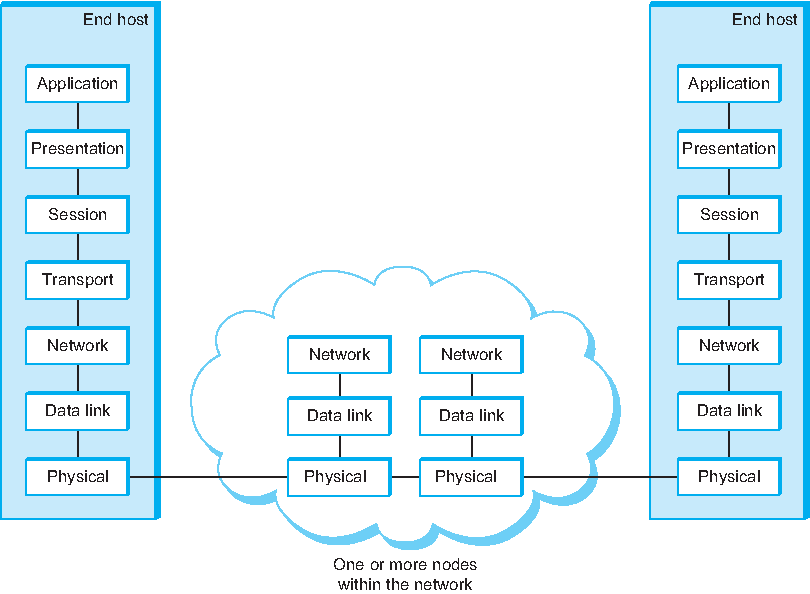
\includegraphics[height=0.75\textheight]{../intro/systemsapproach-1-fig-13.pdf}
};
\coordinate[overlay] (explain loc) at ([yshift=1cm,xshift=0cm]osi.north east);
\tikzset{
    explain box/.style={font=\small,alt=<2>{draw=red}{draw=black},very thick,align=left,at={(explain loc)}, anchor=north west},
    alt explain box/.style={draw=red,ultra thick,anchor=north east,align=left,at={([yshift=-1cm]explain loc)},fill=white},
}
\begin{visibleenv}<2->
\node[overlay,explain box] {
    (7) \myemph<3>{application}: \\ \hspace{.5cm}what requests/etc. \\
    (6) \myemph<3>{presentation}: \\ \hspace{.5cm}data format \\
    (5) \myemph<3>{session}: \\ \hspace{.5cm}manage group of streams \\
    (4) transport: \\ \hspace{.5cm}streams of data \\
    (3) network: \\ \hspace{.5cm}message to correct network \\
    (2) data link: \\ \hspace{.5cm}message $\rightarrow$ bits \\
    \hspace{.5cm}message to correct machine \\
    (1) physical: \\ \hspace{.5cm}send bits/\ldots 
};
\end{visibleenv}
\begin{visibleenv}<3>
\node[overlay,alt explain box] {
    current Internet \\
    usually* layers 5--7 merged together
};
\end{visibleenv}
\end{tikzpicture}
\imagecredit{Figure 13 of Chapter 1 of Computer Networks: A Systems Approach (6th ed) (Peterson and Davie)}
\end{frame}

\begin{frame}<0>{OSI model (text)}
\begin{tabular}{lll} \hline
7 & \myemph<2>{application} & what requests/etc. \\ \hline 
6 & \myemph<2>{presentation} & format of data \\ \hline 
5 & \myemph<2>{session} & coordinate multiple streams \\ \hline
4 & transport & streams of data \\ \hline
3 & network & message to correct network \\ \hline
2 & data link & message to correct machine \\ 
~ & ~ & message into bits/symbols \\
1 & physical & transmit bits/symbols on medium \\
\end{tabular}
\begin{itemize}
\item<2-> \myemph<2>{internet: usually combines layers 7/6/5}
\end{itemize}
\end{frame}

\begin{frame}{OSI model}
    \begin{itemize}
    \item standardized by ISO (International Standards Organization) and ITU (International Telecommunications Union)
    \item full set of protocols\ldots
        \begin{itemize}
        \item file transfer, message sending, directory lookups \ldots
        \end{itemize}
    \item that were often implemented and sometimes used\ldots
    \item but mostly lost out to IETF-standardized Internet protocols
        \begin{itemize}
        \item Internet Engineering Task Force
        \end{itemize}
    \end{itemize}
\end{frame}

\begin{frame}{OSI influence (1)}
    \begin{itemize}
    \item term `layer 7', `layer 4', `layer 3', etc. almost always refer to OSI model
    \item \ldots even though most of Internet does not follow it
        \begin{itemize}
        \item early Internet protocols predate OSI
        \end{itemize}
    \end{itemize}
\end{frame}

\begin{frame}{OSI influence (2)}
    \begin{itemize}
    \item are a lot of Internet protocols influenced by OSI protocols
    \vspace{.5cm}
    \item OSI's DAP (directory access protocol) 
        \begin{itemize}
        \item adapted into IETF's LDAP (lightweight directory access protocol)
        \end{itemize}
    \item OSI presentation layer ASN.1 used in\ldots
        \begin{itemize}
        \item telephony (between telephone companies)
        \item inter-bank messaging
        \item lots of cryptography-related protocols
        \item \ldots
        \end{itemize}
    \item OSI's routing protocol IS-IS still common in large Internet-connected networks
        \begin{itemize}
        \item (adapted to work alongside IETF protocols)
        \end{itemize}
    \end{itemize}
\end{frame}

\begin{frame}{Internet layers}
\small
\begin{tabular}{|l|l|l|p{6cm}|} 
OSI layer & name & examples & purpose \\ \hline
7 & application & HTTP, SSH, & {application-defined meanings}\\
~ & ~ & SMTP, DNS, \ldots & ~ \\ \hline
4 & {transport} & TCP, UDP, \ldots & {reach correct program,\linebreak \myemph<2>{reliablity/streams}} \\ \hline
3 & {network} & IPv4, IPv6, \ldots & {reach correct machine}\linebreak(across networks) \\ \hline
2 & {link} & Ethernet, Wi-Fi, \ldots & {coordinate shared wire/radio}\\ \hline
1 & physical & \ldots & encode bits for wire/radio \\ \hline
\end{tabular}
\end{frame}

\begin{frame}{Internet protocols and layers (non-exhaustive)}
\begin{tikzpicture}
\node[anchor=north west] (int) at (0,0) {
    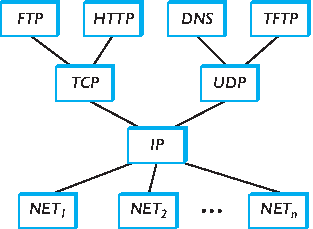
\includegraphics[height=0.75\textheight]{../intro/systemsapproach-1-fig-14.pdf}
};
%\draw[help lines] (0, 0) grid (14, -8);
%\draw[step=2,draw,thick,red] (0, 0) grid (14, -8);
\tikzset{
    layer hi/.style={draw=red,ultra thick},
    layer label/.style={anchor=west},
}
\draw[layer hi] (0, 0) rectangle (9, -1.3);
\node[layer label] at (9.1, -0.65) { application {\it\small OSI layer 7} };
\draw[layer hi] (1.5, -1.8) rectangle (7.5, -3.2);
\node[layer label] at (8.6, -2.5) { transport {\it\small OSI layer 4} };
\draw[layer hi,alt=<2>{fill=red,fill opacity=0.1}] (3.5, -3.6) rectangle (5.6, -4.85);
\node[layer label] at (5.8, -4.2) (net label) { network {\it\small OSI layer 3} };
\draw[layer hi] (0.5, -5.5) rectangle (9, -6.6);
\node[layer label] at (9.1, -6) { data link {\it\small OSI layer 2} };
\begin{visibleenv}<2>
    \node[anchor=west,red,font=\large] at (net label.east) {``narrow waist''};
\end{visibleenv}
\end{tikzpicture}
\imagecredit{Figure 14 of Chapter 1 of Computer Networks: A Systems Approach (6th ed) (Peterson and Davie)}
\end{frame}





\section{physical layer: synchronizing}



\begin{frame}{Manchester encoding}
\begin{tikzpicture}
\node (fig) { 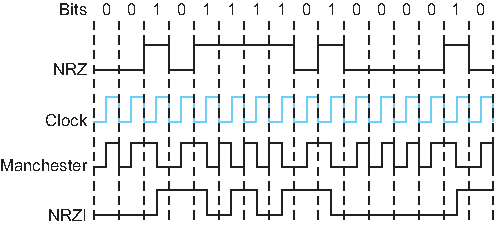
\includegraphics[width=0.9\textwidth]{../physical/SysApproach-2-Fig-25.pdf} };
\end{tikzpicture}
\imagecredit{Figure 25 from Section 2.2 of \textit{Computer Networks: A Systems Approach} (6th ed) (Peterson and Davie)}
\end{frame}

\begin{frame}{problem with Manchester}
    \begin{itemize}
    \item fixed the problem of too few transitions
    \vspace{.5cm}
    \item but now most transitions don't send information
    \item means we aren't making good use of wire/etc. capacity
    \vspace{.5cm}
    \item there are more clever compromises
        \begin{itemize}
        \item (example: 4B5B encoding)
        \end{itemize}
    \end{itemize}
\end{frame}

\begin{frame}{other better encoding options}
    \begin{itemize}
    \item vary more than just one thing
        \begin{itemize}
        \item example: pulse amplitude and duration
        \end{itemize}
    \item use more than just low/high
    \item \ldots much more
    \vspace{.5cm}
    \item probably covered in ECE Signals course?
    \end{itemize}
\end{frame}



\end{document}
